\chapter{Anleitung}
Es gibt zwei verschiedene Modi, welche rechts oben am Bildschirmrand gewechselt werden k�nnen. Das Programm startet im Show-Modus, was bedeutet, dass der Editor angezeigt wird. Dort k�nnen B�ume angelegt, bearbeitet und gespeichert werden. Im Hide-Modus k�nnen bereits abgespeicherte B�ume den Robotern zugewiesen werden, da der Editor versteckt wird.

\textbf{{\large Show:}} Editor ist eingeblendet
\section{Anlegen}
Um einen neuen Baum zu erstellen, wird der New-Button gedr�ckt. Daraufhin erscheint ein Fenster mit einer Liste. Dort wird der erste Knoten des Baumes ausgew�hlt.
\begin{figure}[h!] %[hbtp]
	\centering
		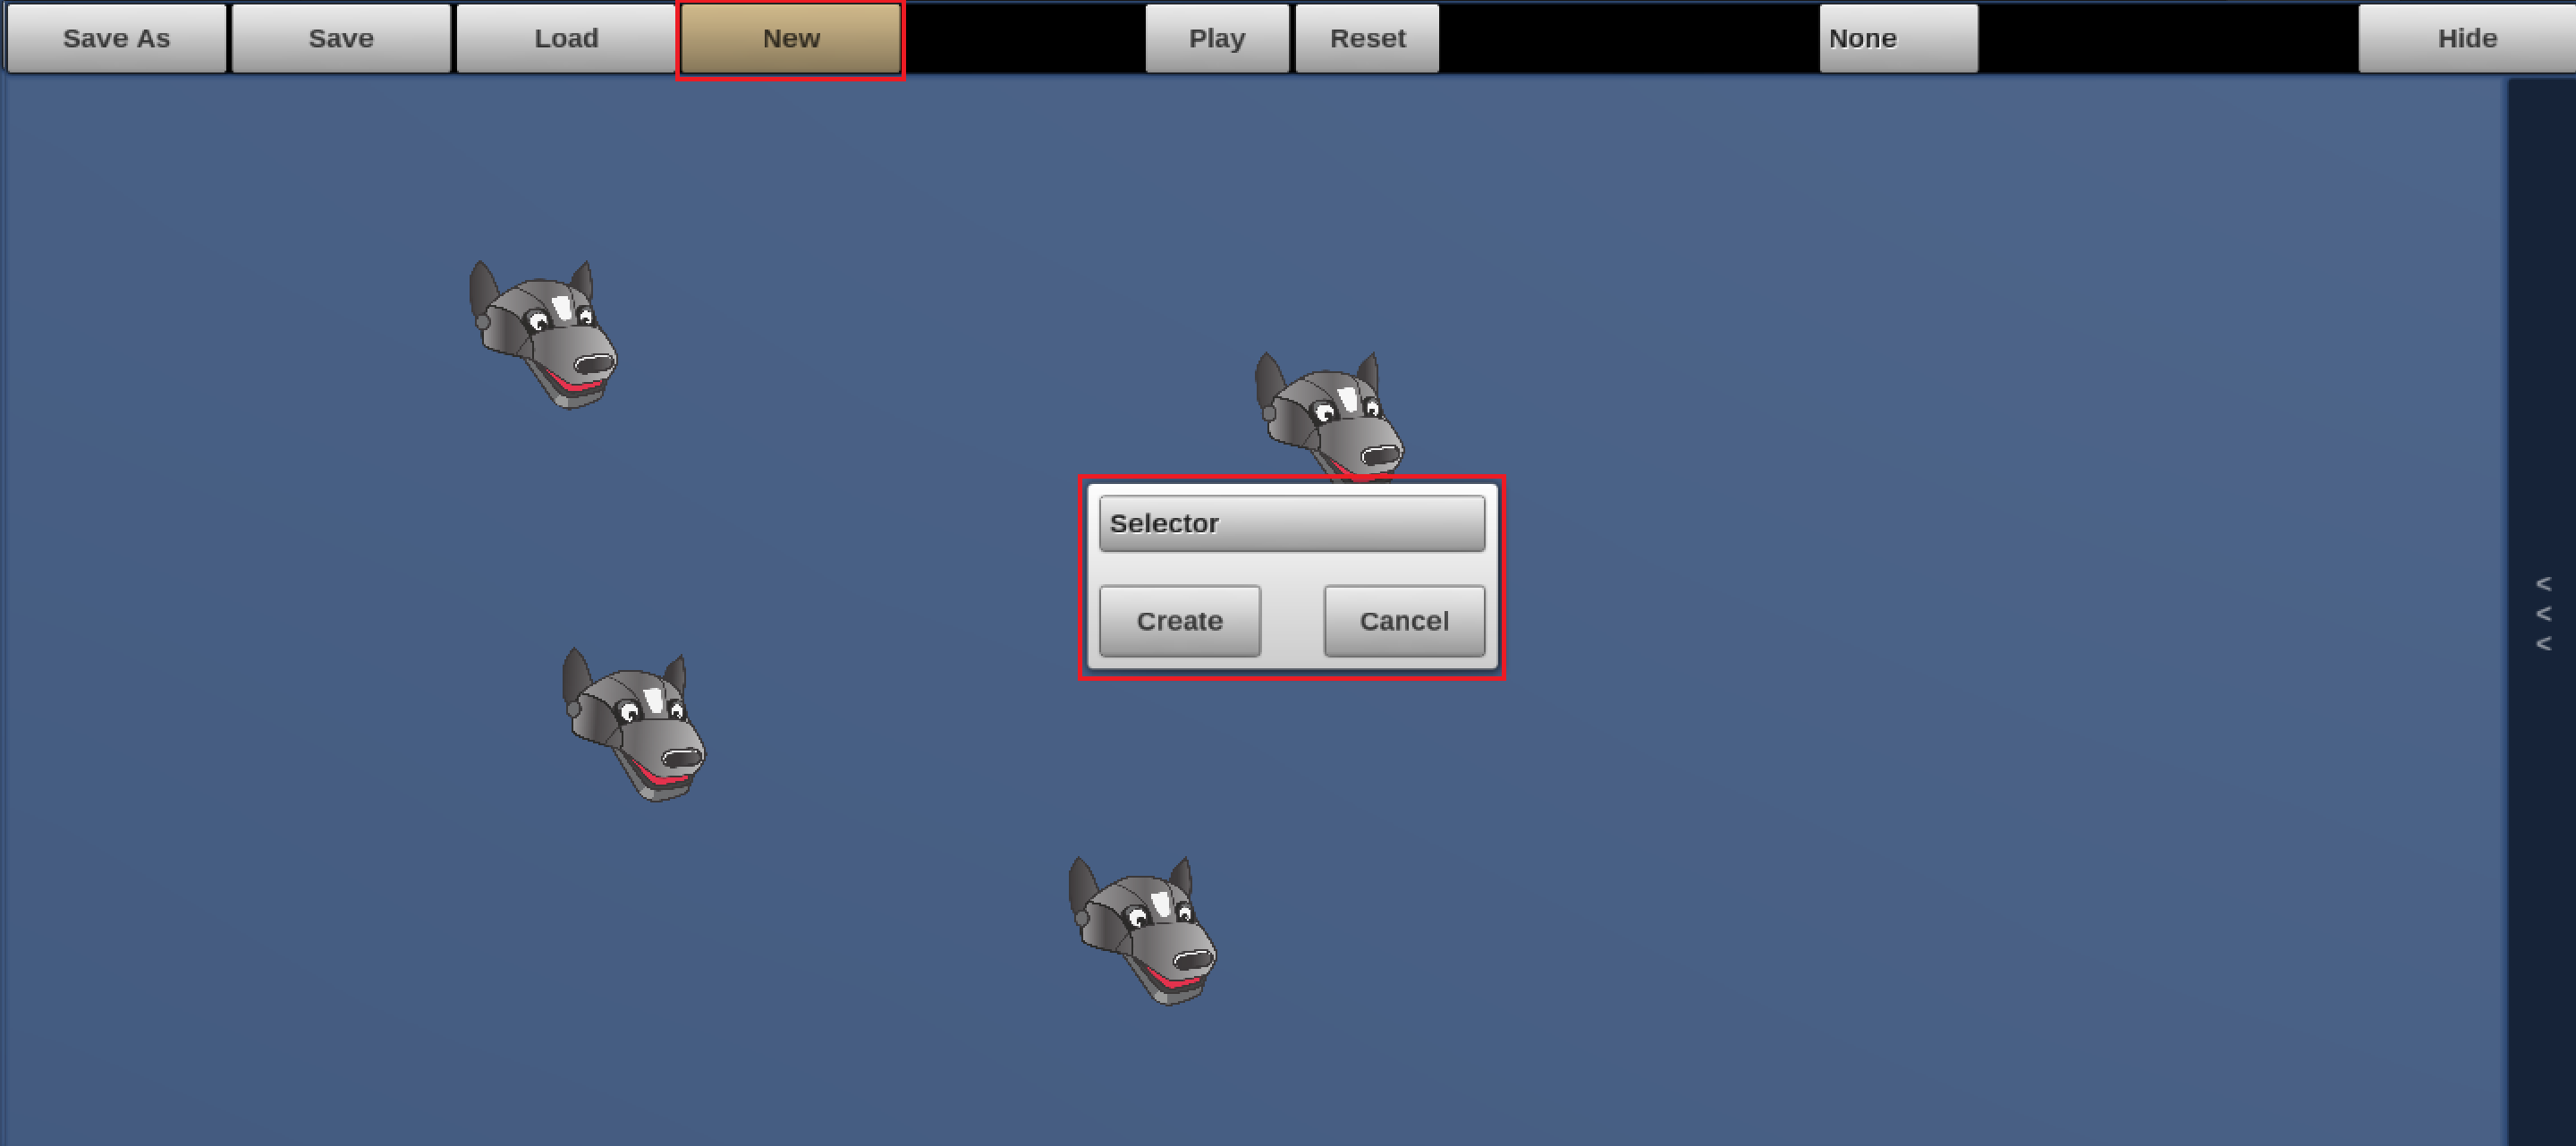
\includegraphics[width=1\textwidth]{images/KIAnleitung3_1}
	\caption{Neuen Baum anlegen}
	\label{a2}
\end{figure}



\section{Bearbeiten}
Am rechten Rand verbirgt sich das Bearbeitungs-Men�. Mit einem Klick auf den schmalen Balken klappt sich dieses auf.

\begin{figure}[h!] %[hbtp]
	\centering
		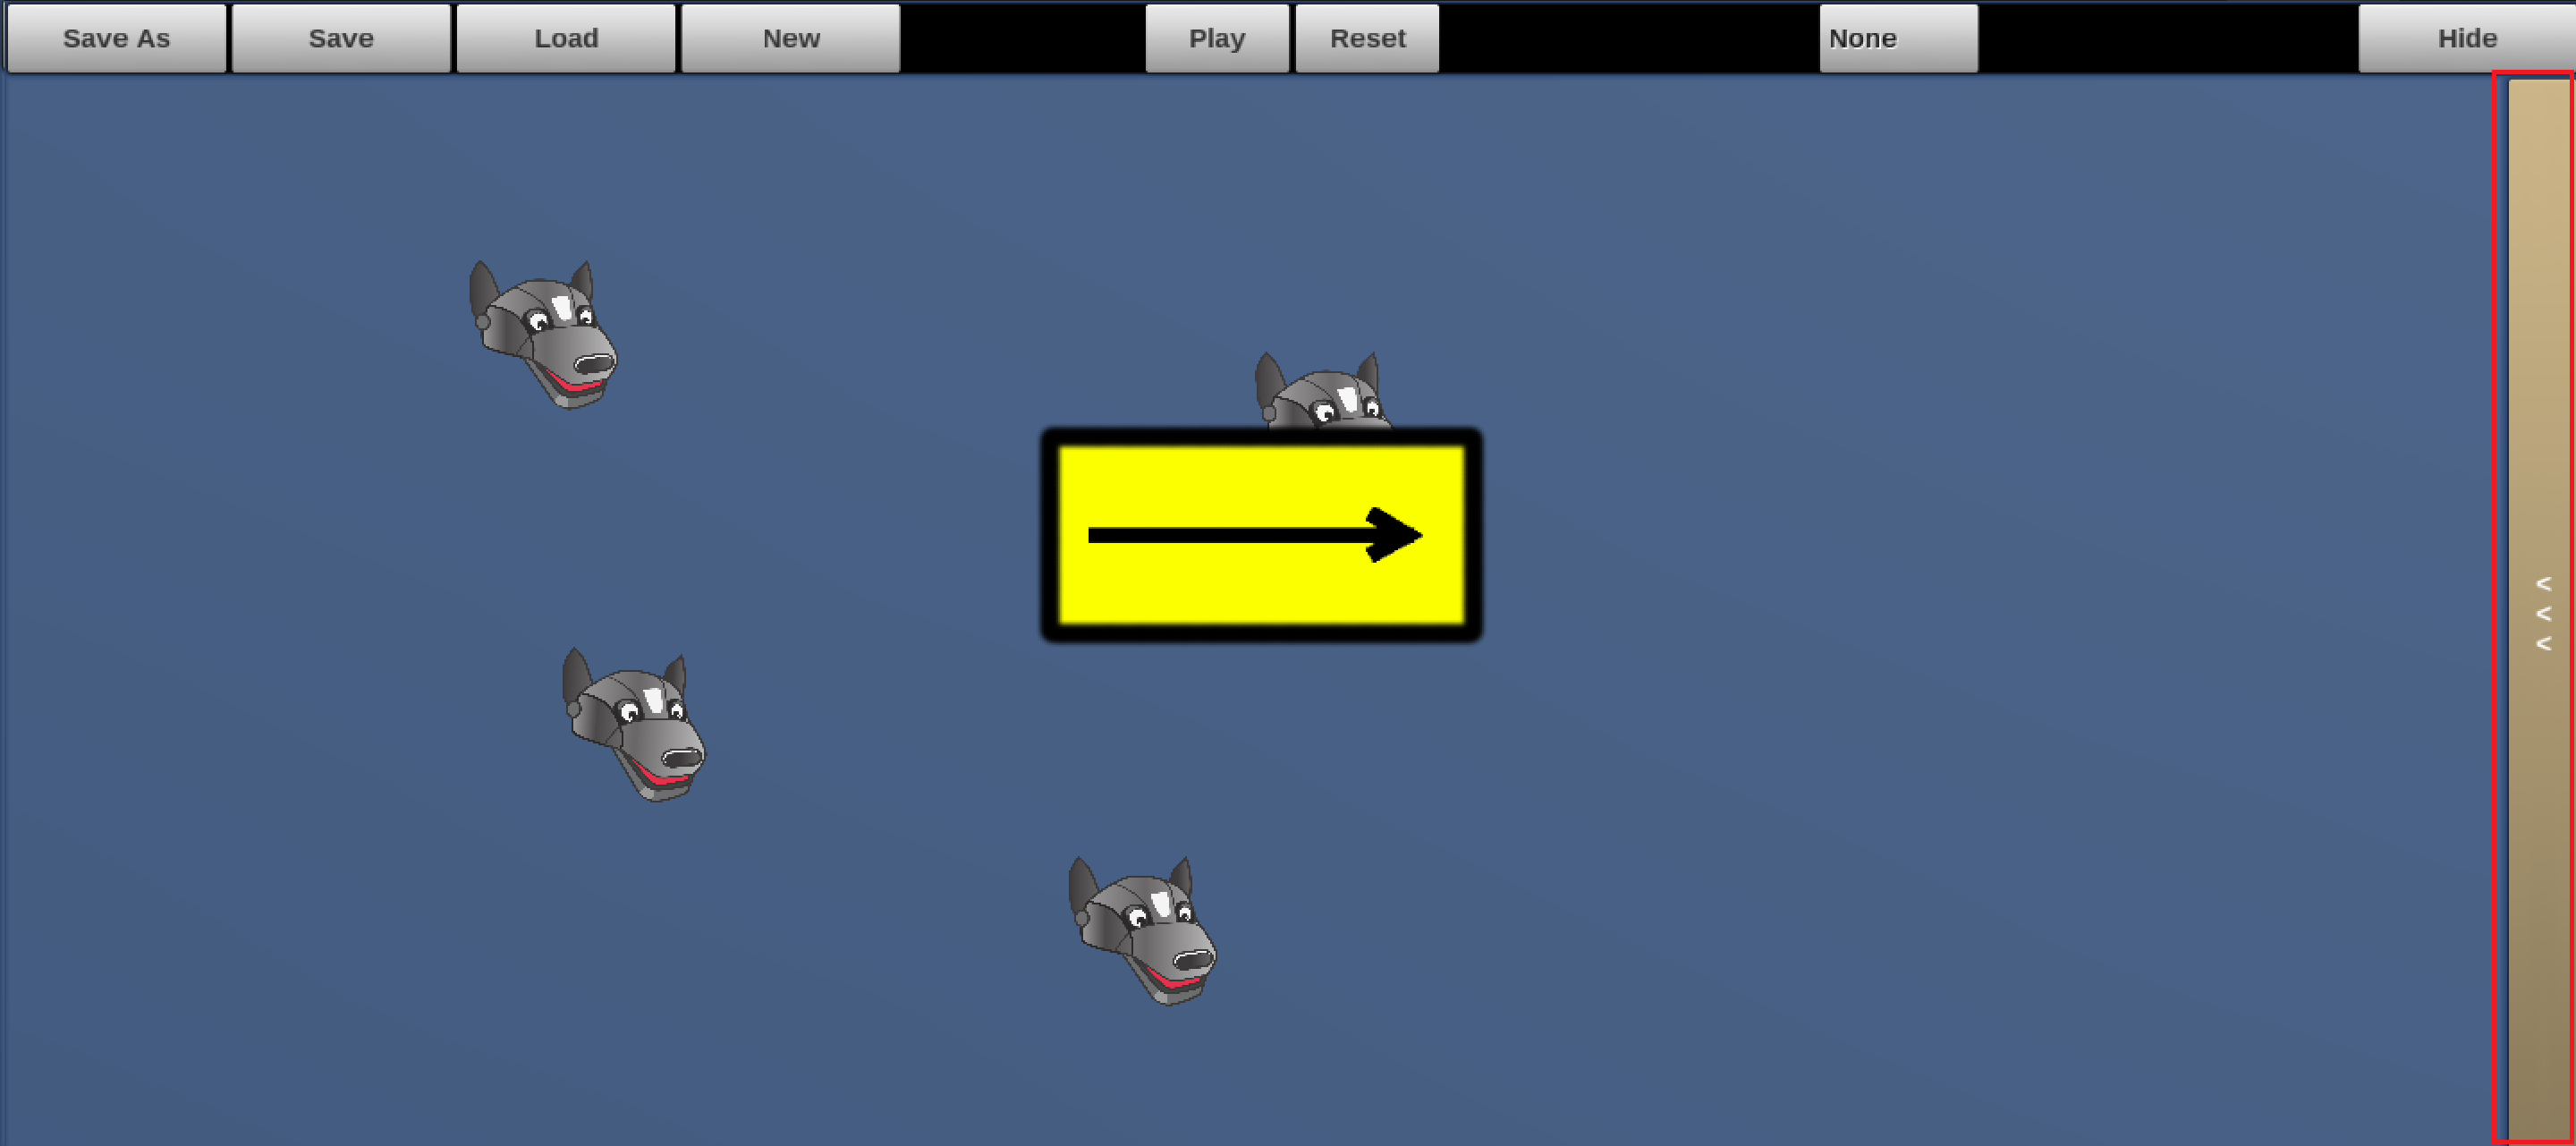
\includegraphics[width=1\textwidth]{images/KIAnleitung4_1}
	\caption{Der Editor ist am rechten Rand eingefahren}
	\label{a3}
\end{figure}

\section{Knoten Ausw�hlen}
Mit einem Klick auf den zu bearbeitenden Knoten direkt im Baum wird dieser direkt ausgew�hlt und ist dadurch bearbeitbar.

\begin{figure}[h!] %[hbtp]
	\centering
		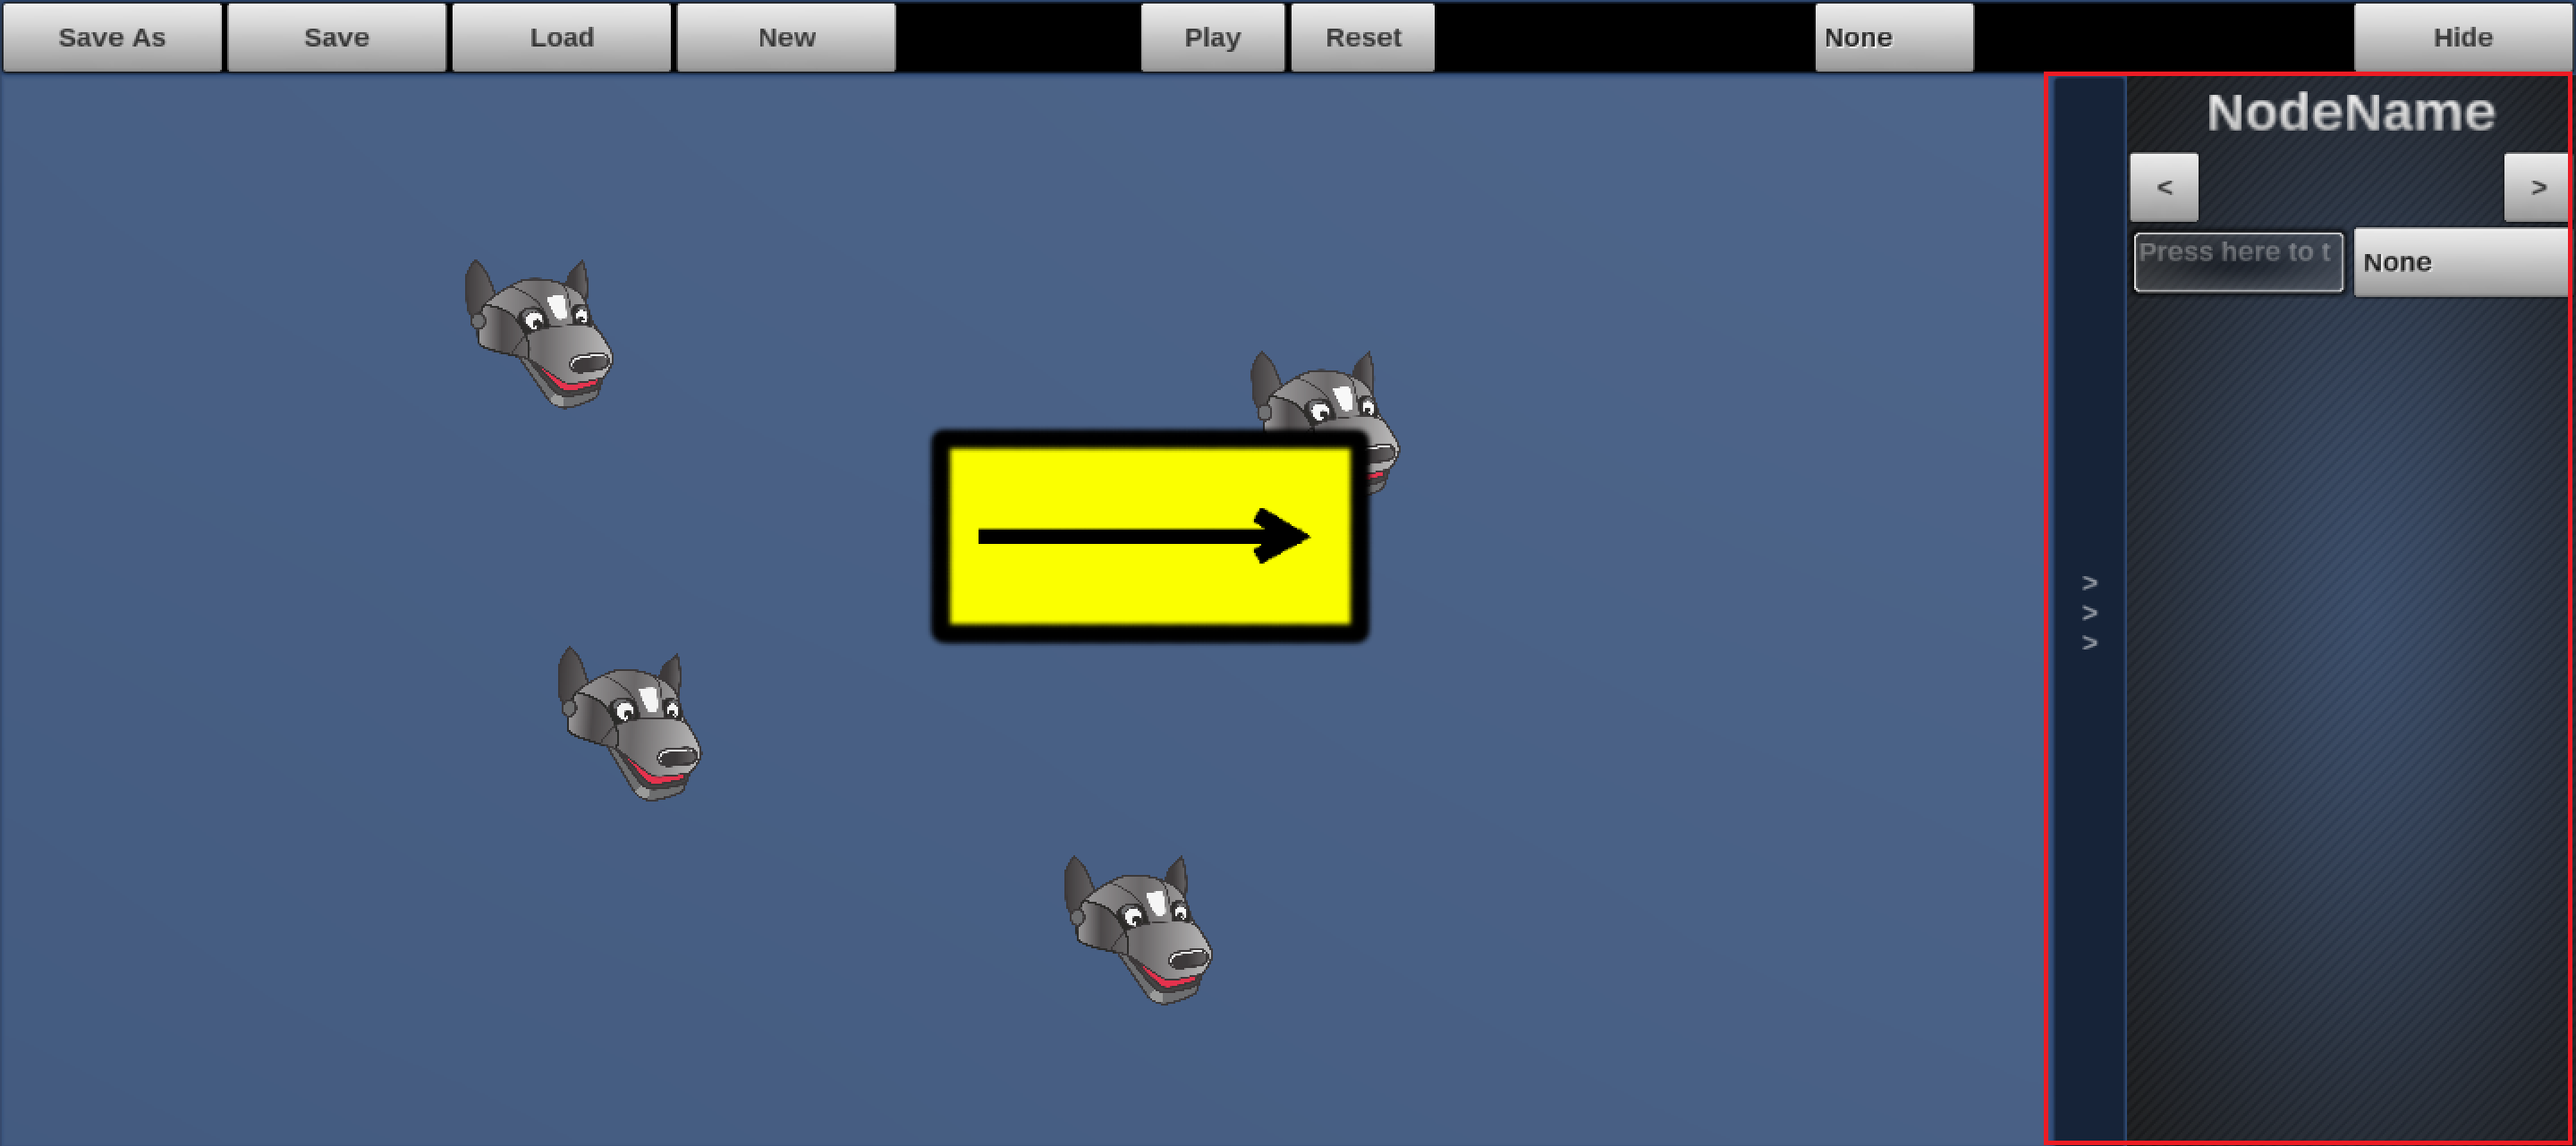
\includegraphics[width=1\textwidth]{images/KIAnleitung5_1}
	\caption{Der Knotenname und die Unterknoten werden angezeigt}
	\label{a4}
\end{figure}

\section{Unterknoten anlegen}
Wenn ein Vaterknoten ausgew�hlt ist, l�sst sich �ber die Liste im Bearbeitungsfenster ein neuer Task als Unterknoten hinzuf�gen. Zum Einzuschr�nken der Liste dient die Suchfunktion, welche auf Gro�- und Kleinschreibung achtet.

\begin{figure}[h!] %[hbtp]
	\centering
		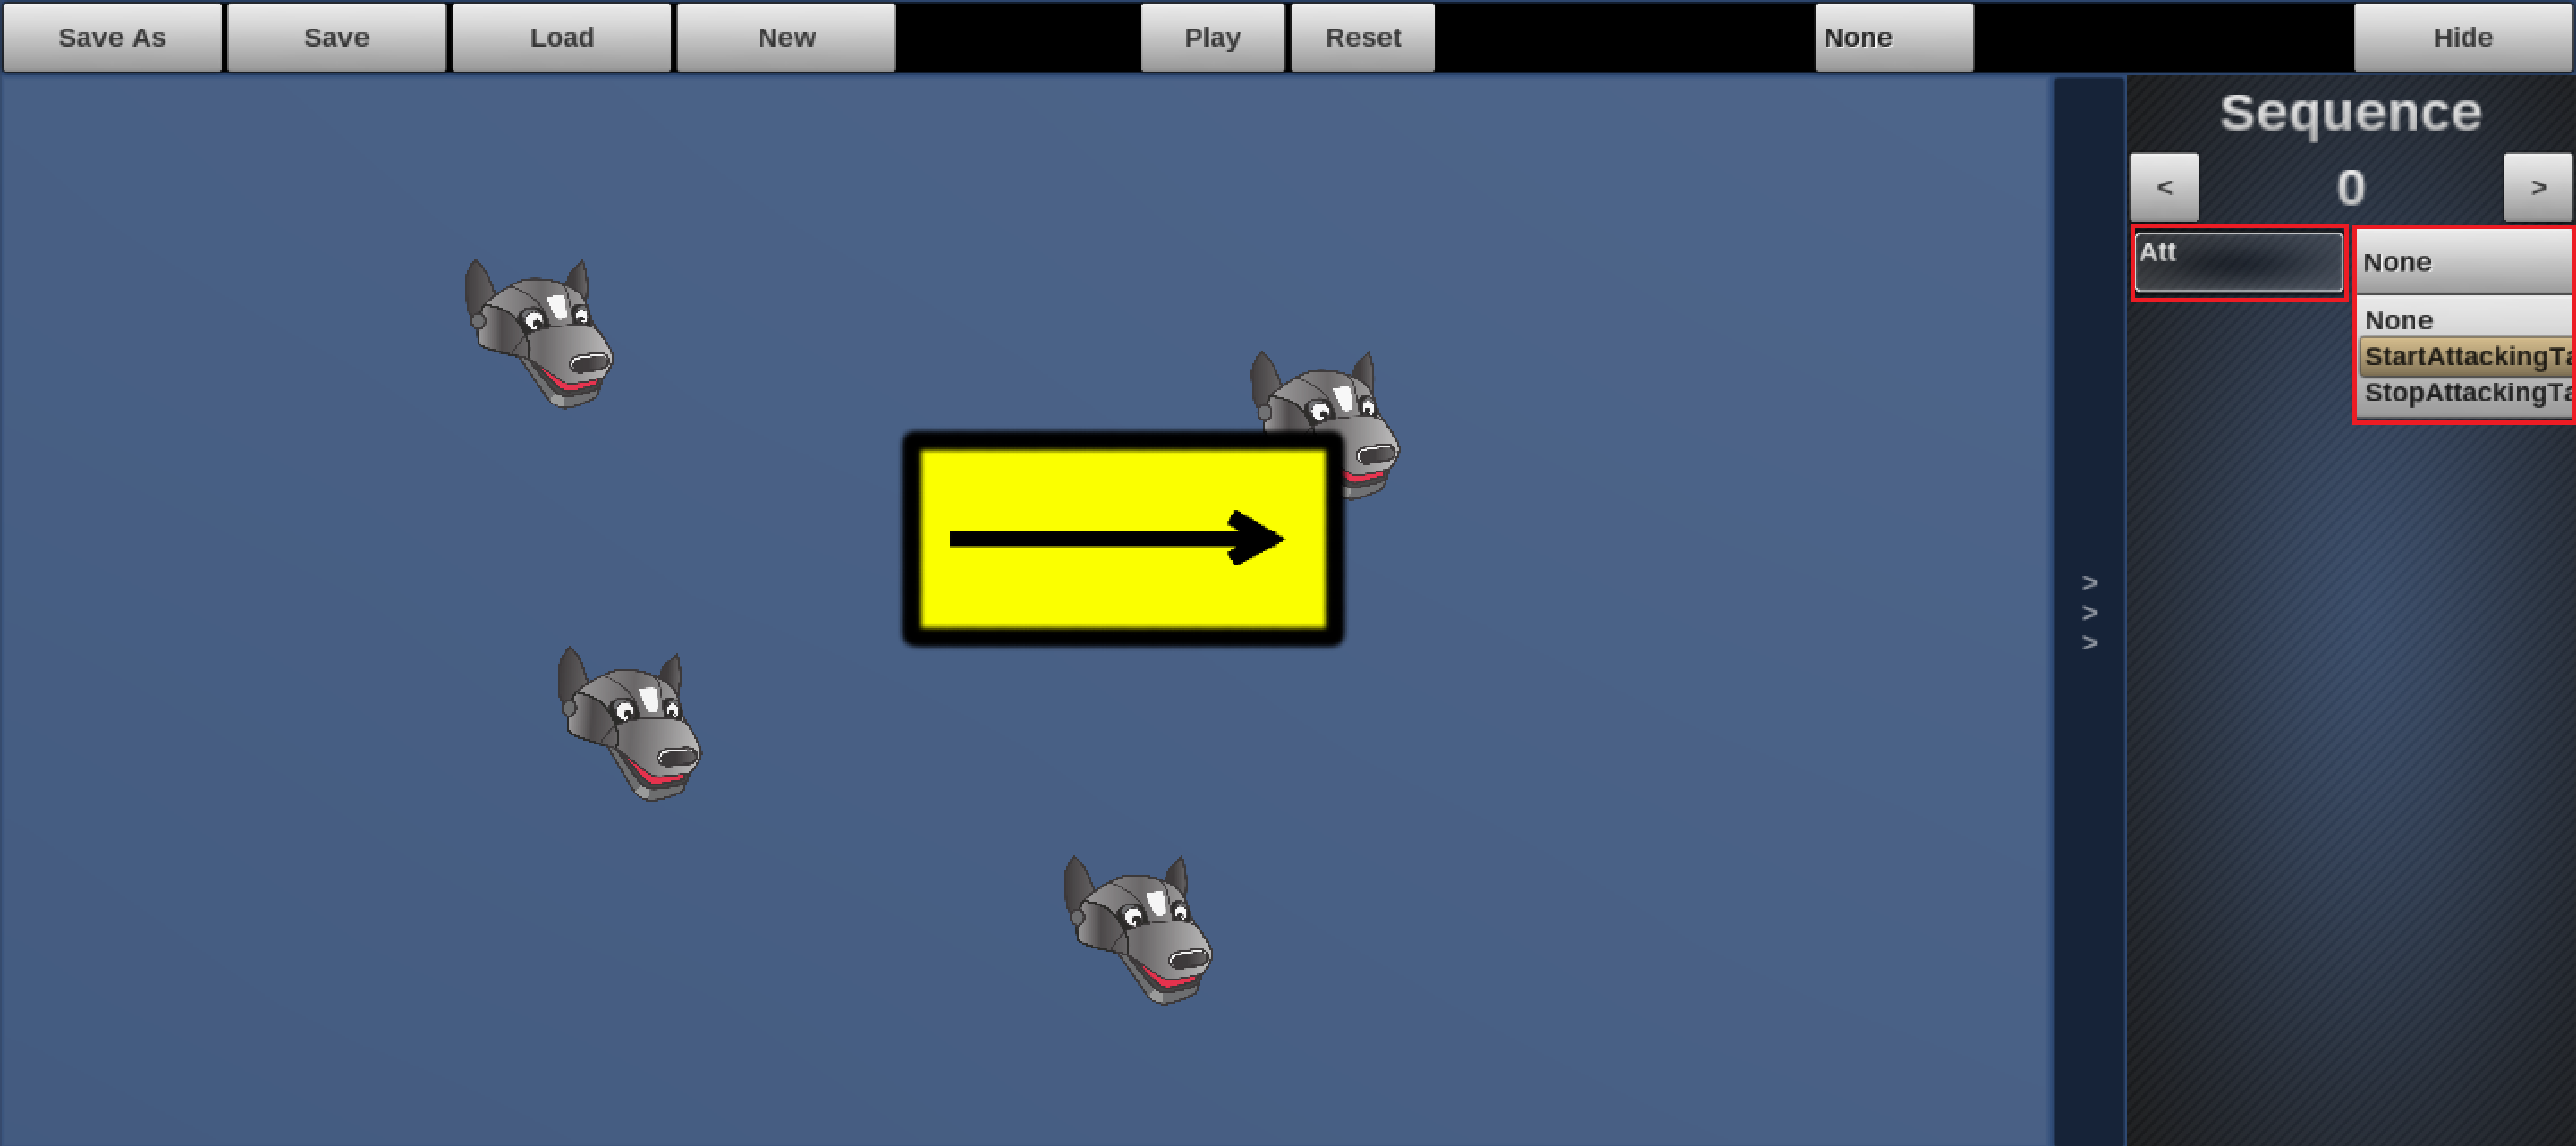
\includegraphics[width=1\textwidth]{images/KIAnleitung55_1}
	\caption{Suchfenster und eine Liste von gefundenen Tasks}
	\label{a5}
\end{figure}

\begin{figure}[h!] %[hbtp]
	\centering
		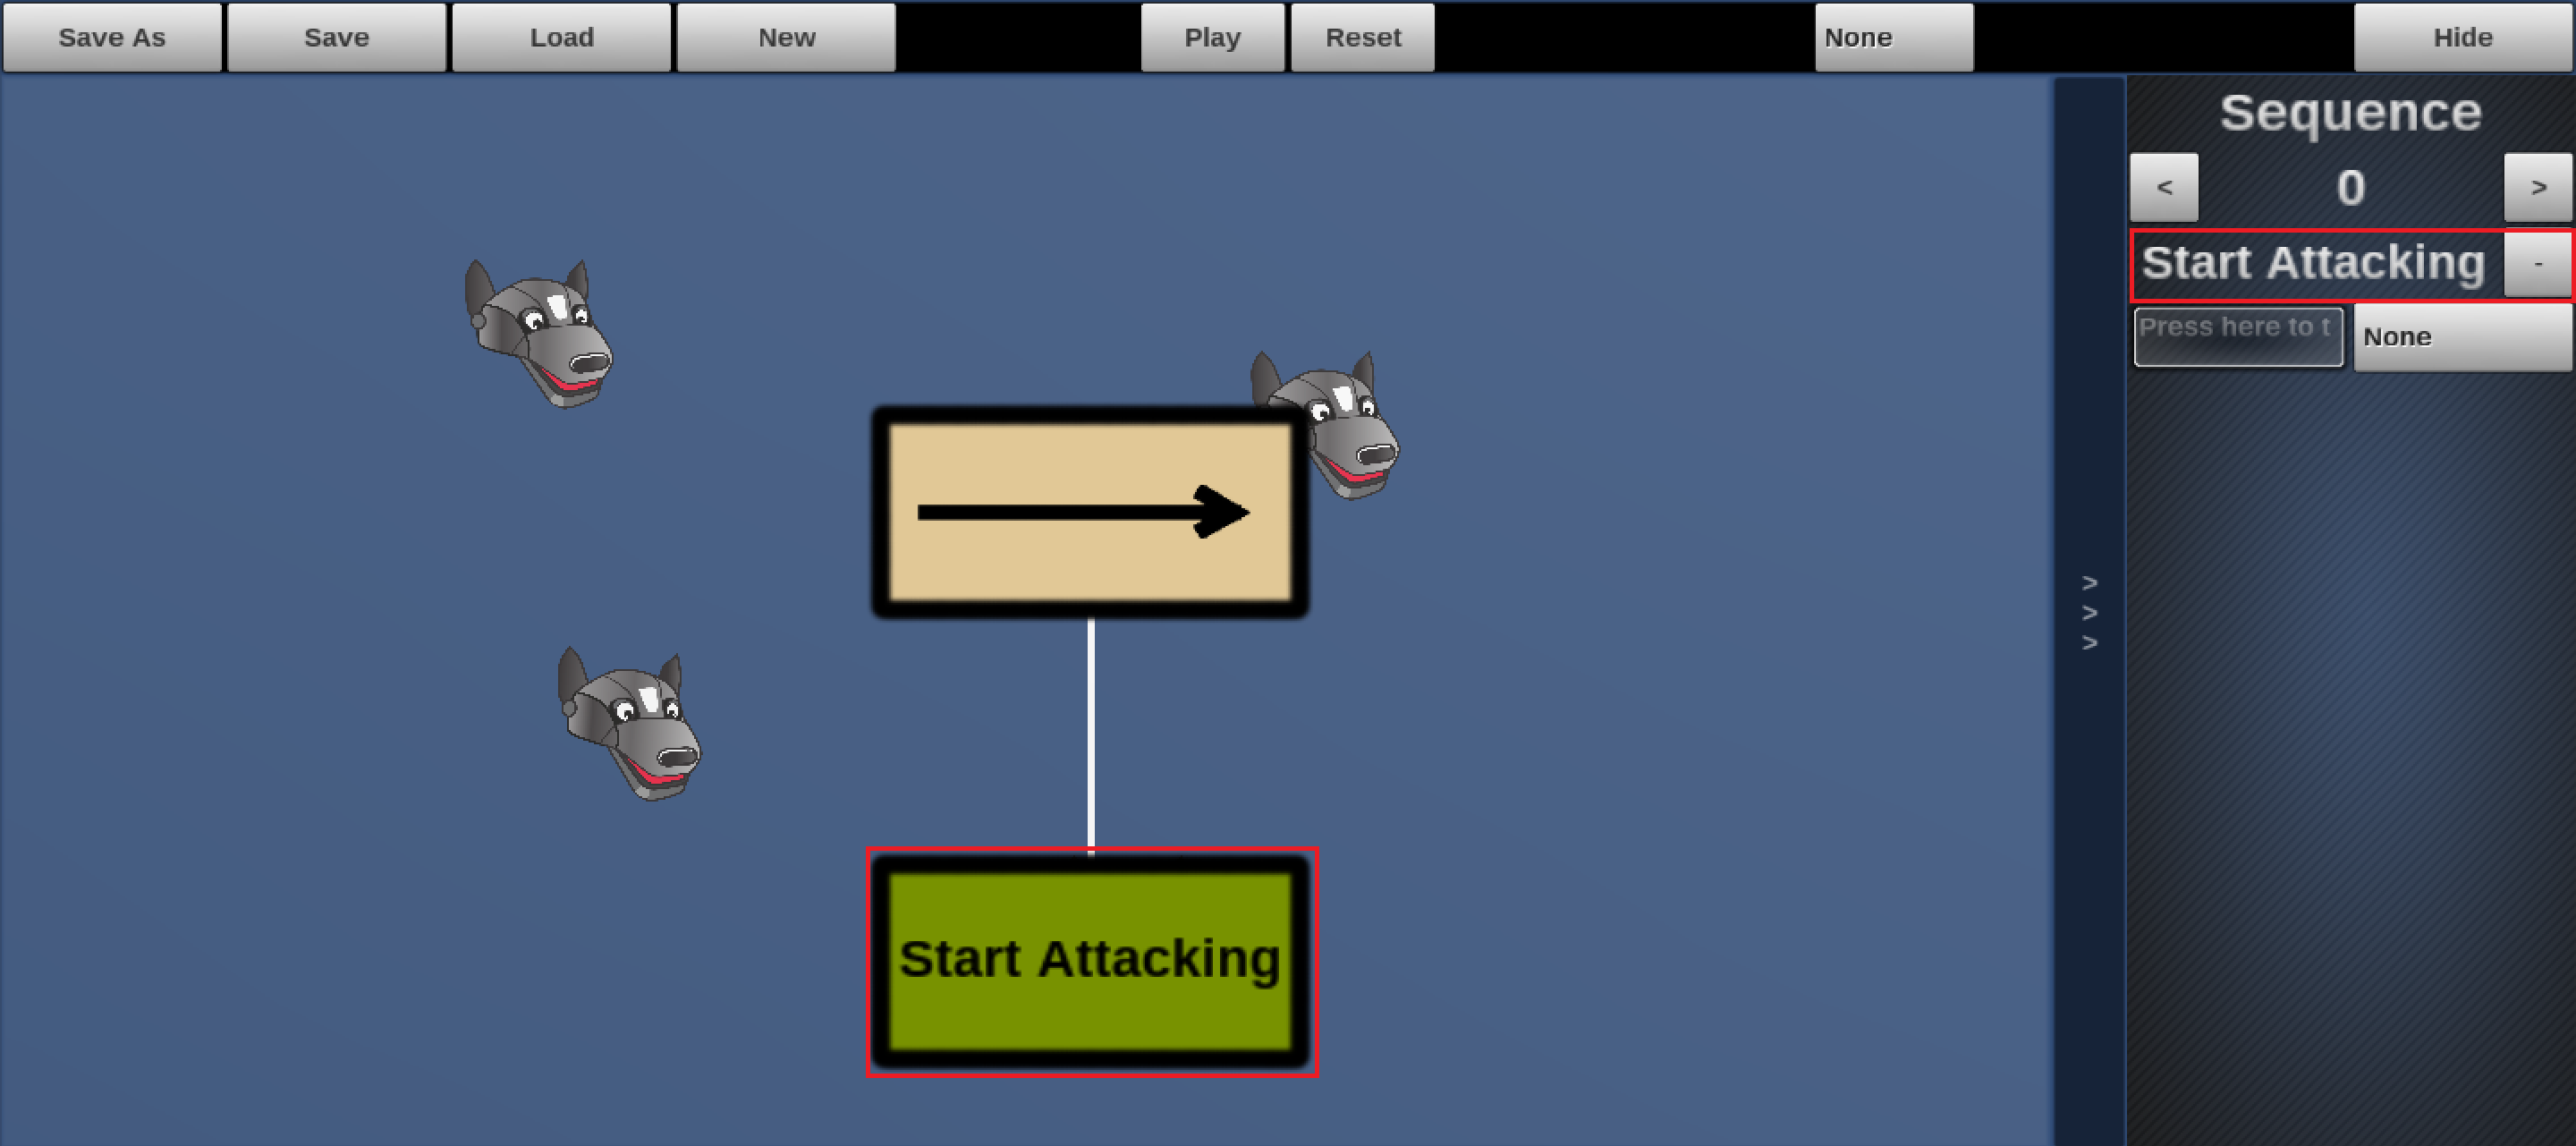
\includegraphics[width=1\textwidth]{images/KIAnleitung555_1}
	\caption{Neuer Kindknoten wurde angelegt}
	\label{a6}
\end{figure}


\newpage
\section{Knoten verschieben}
Direkt unter dem Namen des Knotens befindet sich die Index-Position des Konten in der Reihe der Unterknoten. Mit einem Klick auf den Links- oder Rechts-Button wird der Knoten in der Reihe dementsprechend verschoben.
\begin{figure}[h!] %[hbtp]
	\centering
		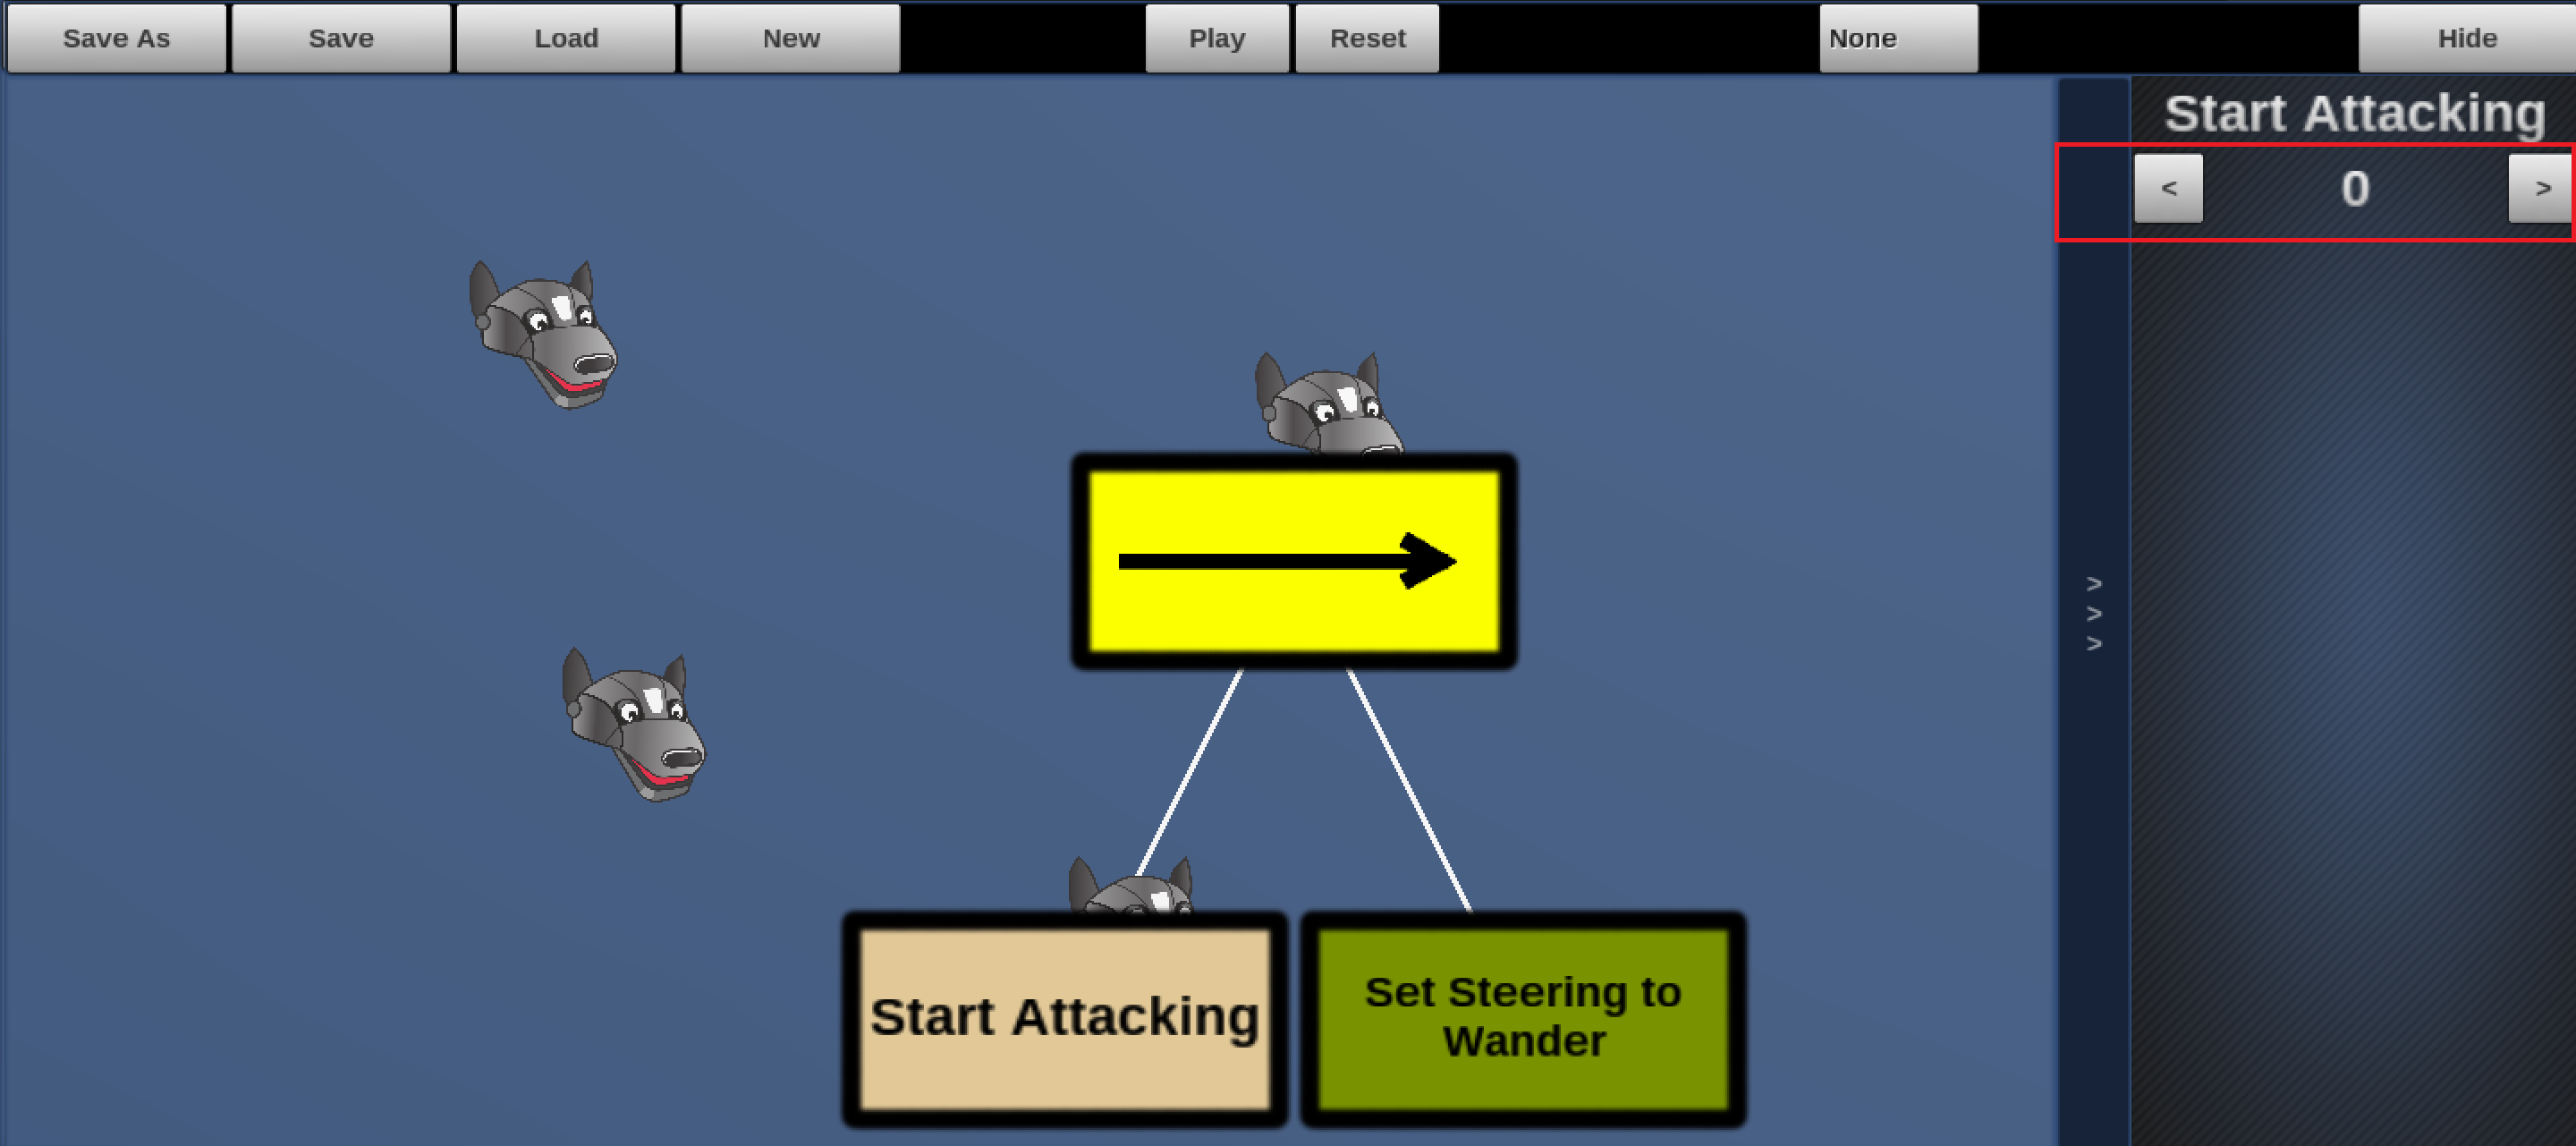
\includegraphics[width=1\textwidth]{images/KIAnleitung6_1}
	\caption{Verschiebung �ber die Index-Pfeile}
	\label{a7}
\end{figure}

\begin{figure}[h!] %[hbtp]
	\centering
		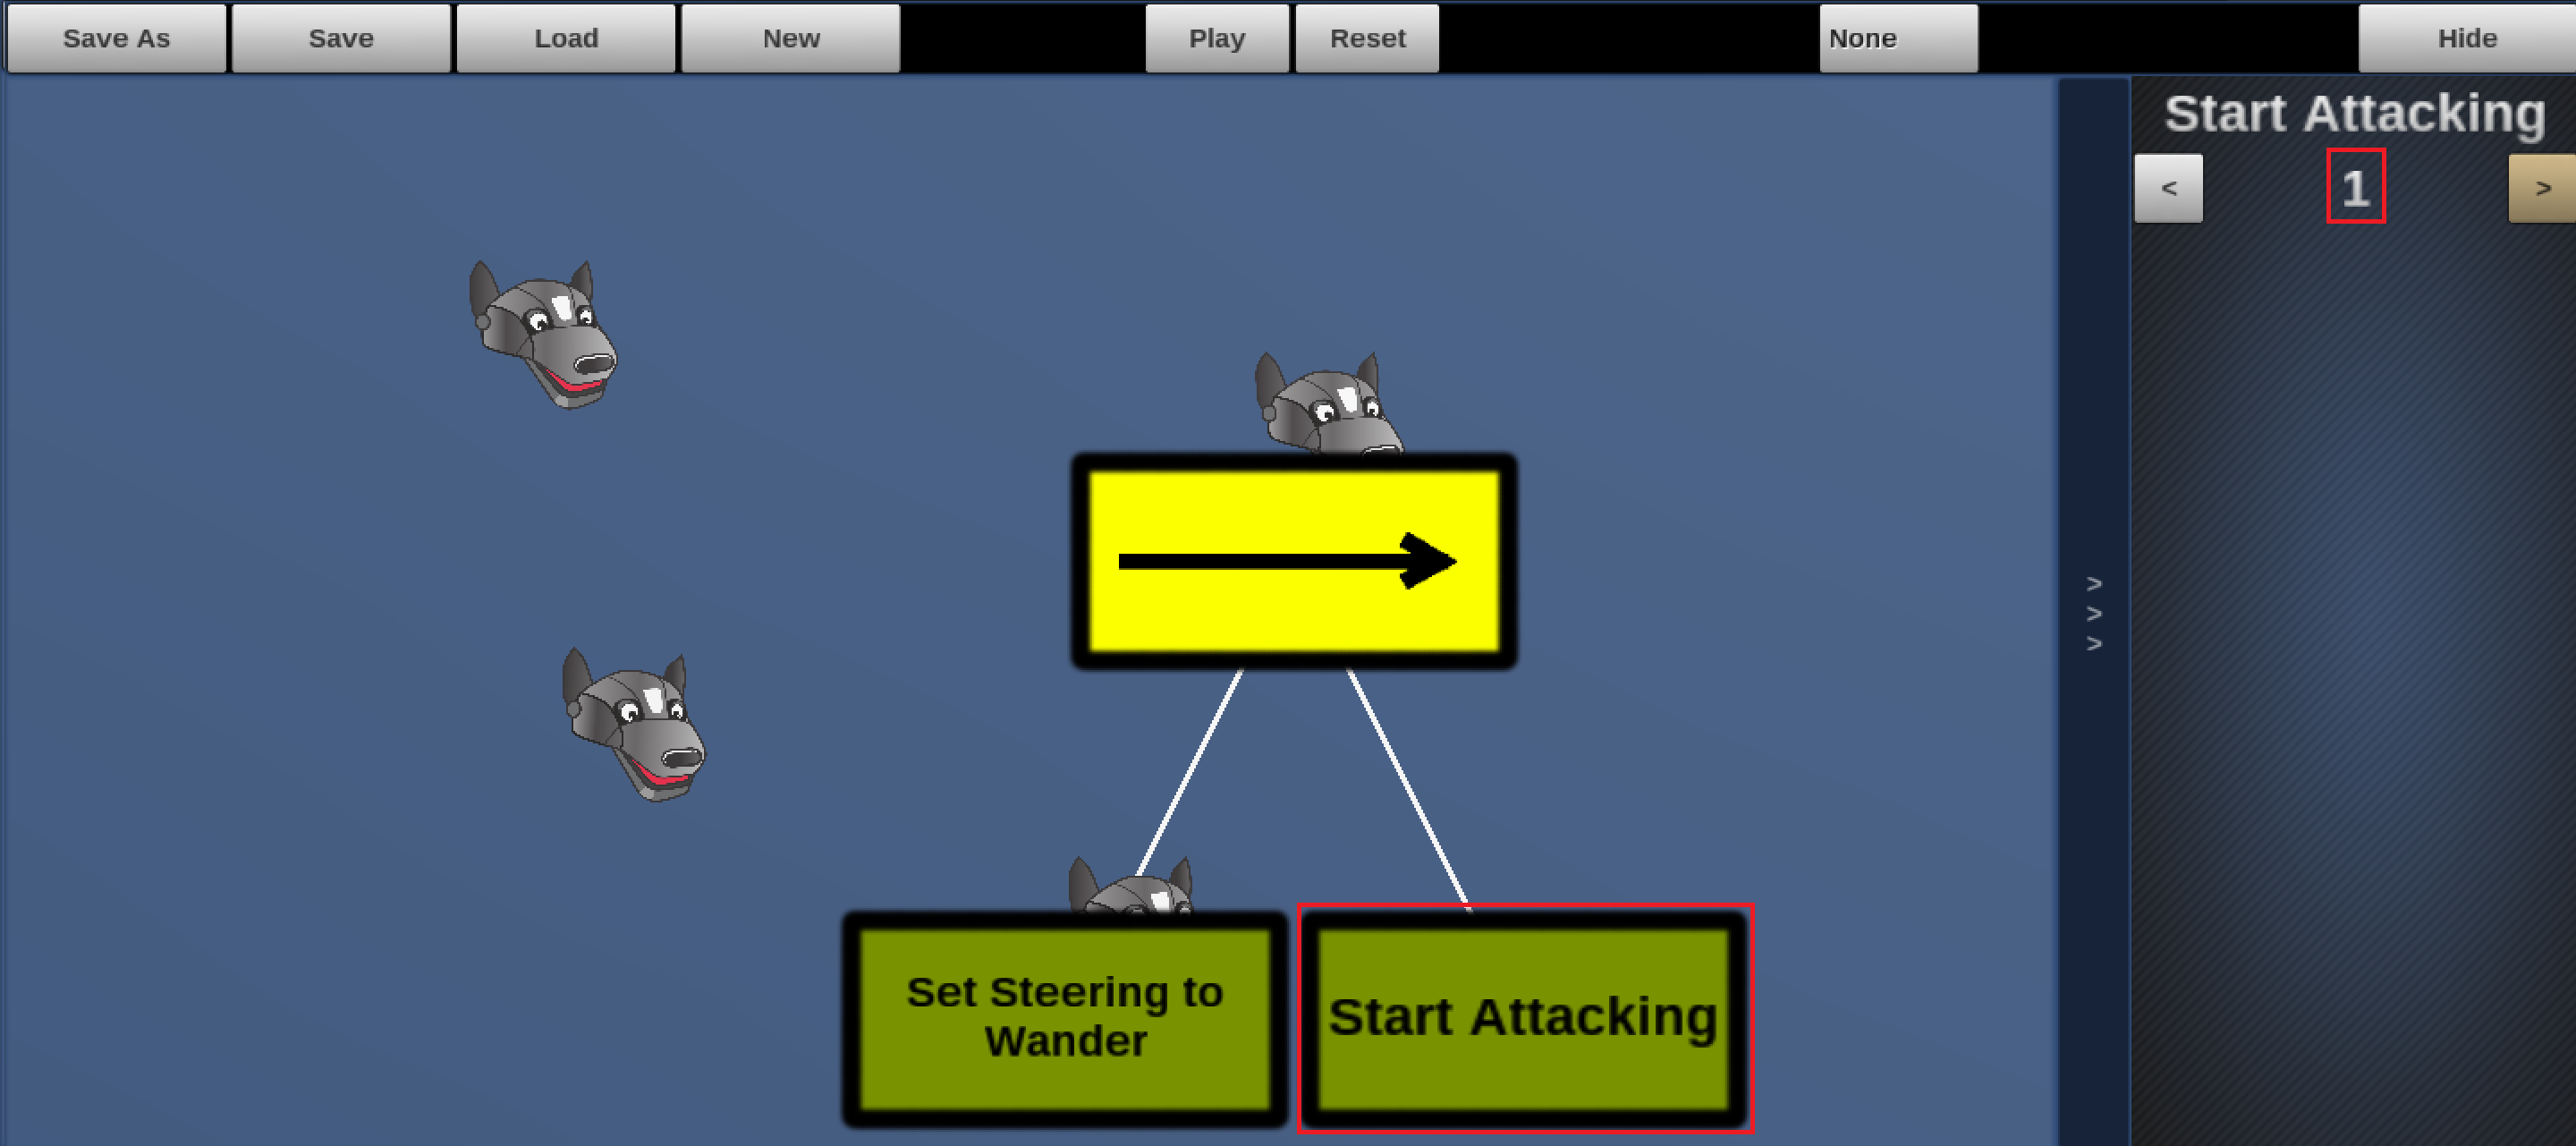
\includegraphics[width=1\textwidth]{images/KIAnleitung7_1}
	\caption{Position wird aktualisiert}
	\label{a8}
\end{figure}

\newpage
\section{Knoten l�schen}
Um einen Knoten zu l�schen, wird der Vaterknoten dessen ausgew�hlt. Dort stehen die Kind-Knoten aufgelistet. Rechts neben den Namen dieser befindet sich der L�schen-Button. Durch das Anklicken wird der Knoten aus der Liste der Kindknoten entfernt.
\begin{figure}[h!] %[hbtp]
	\centering
		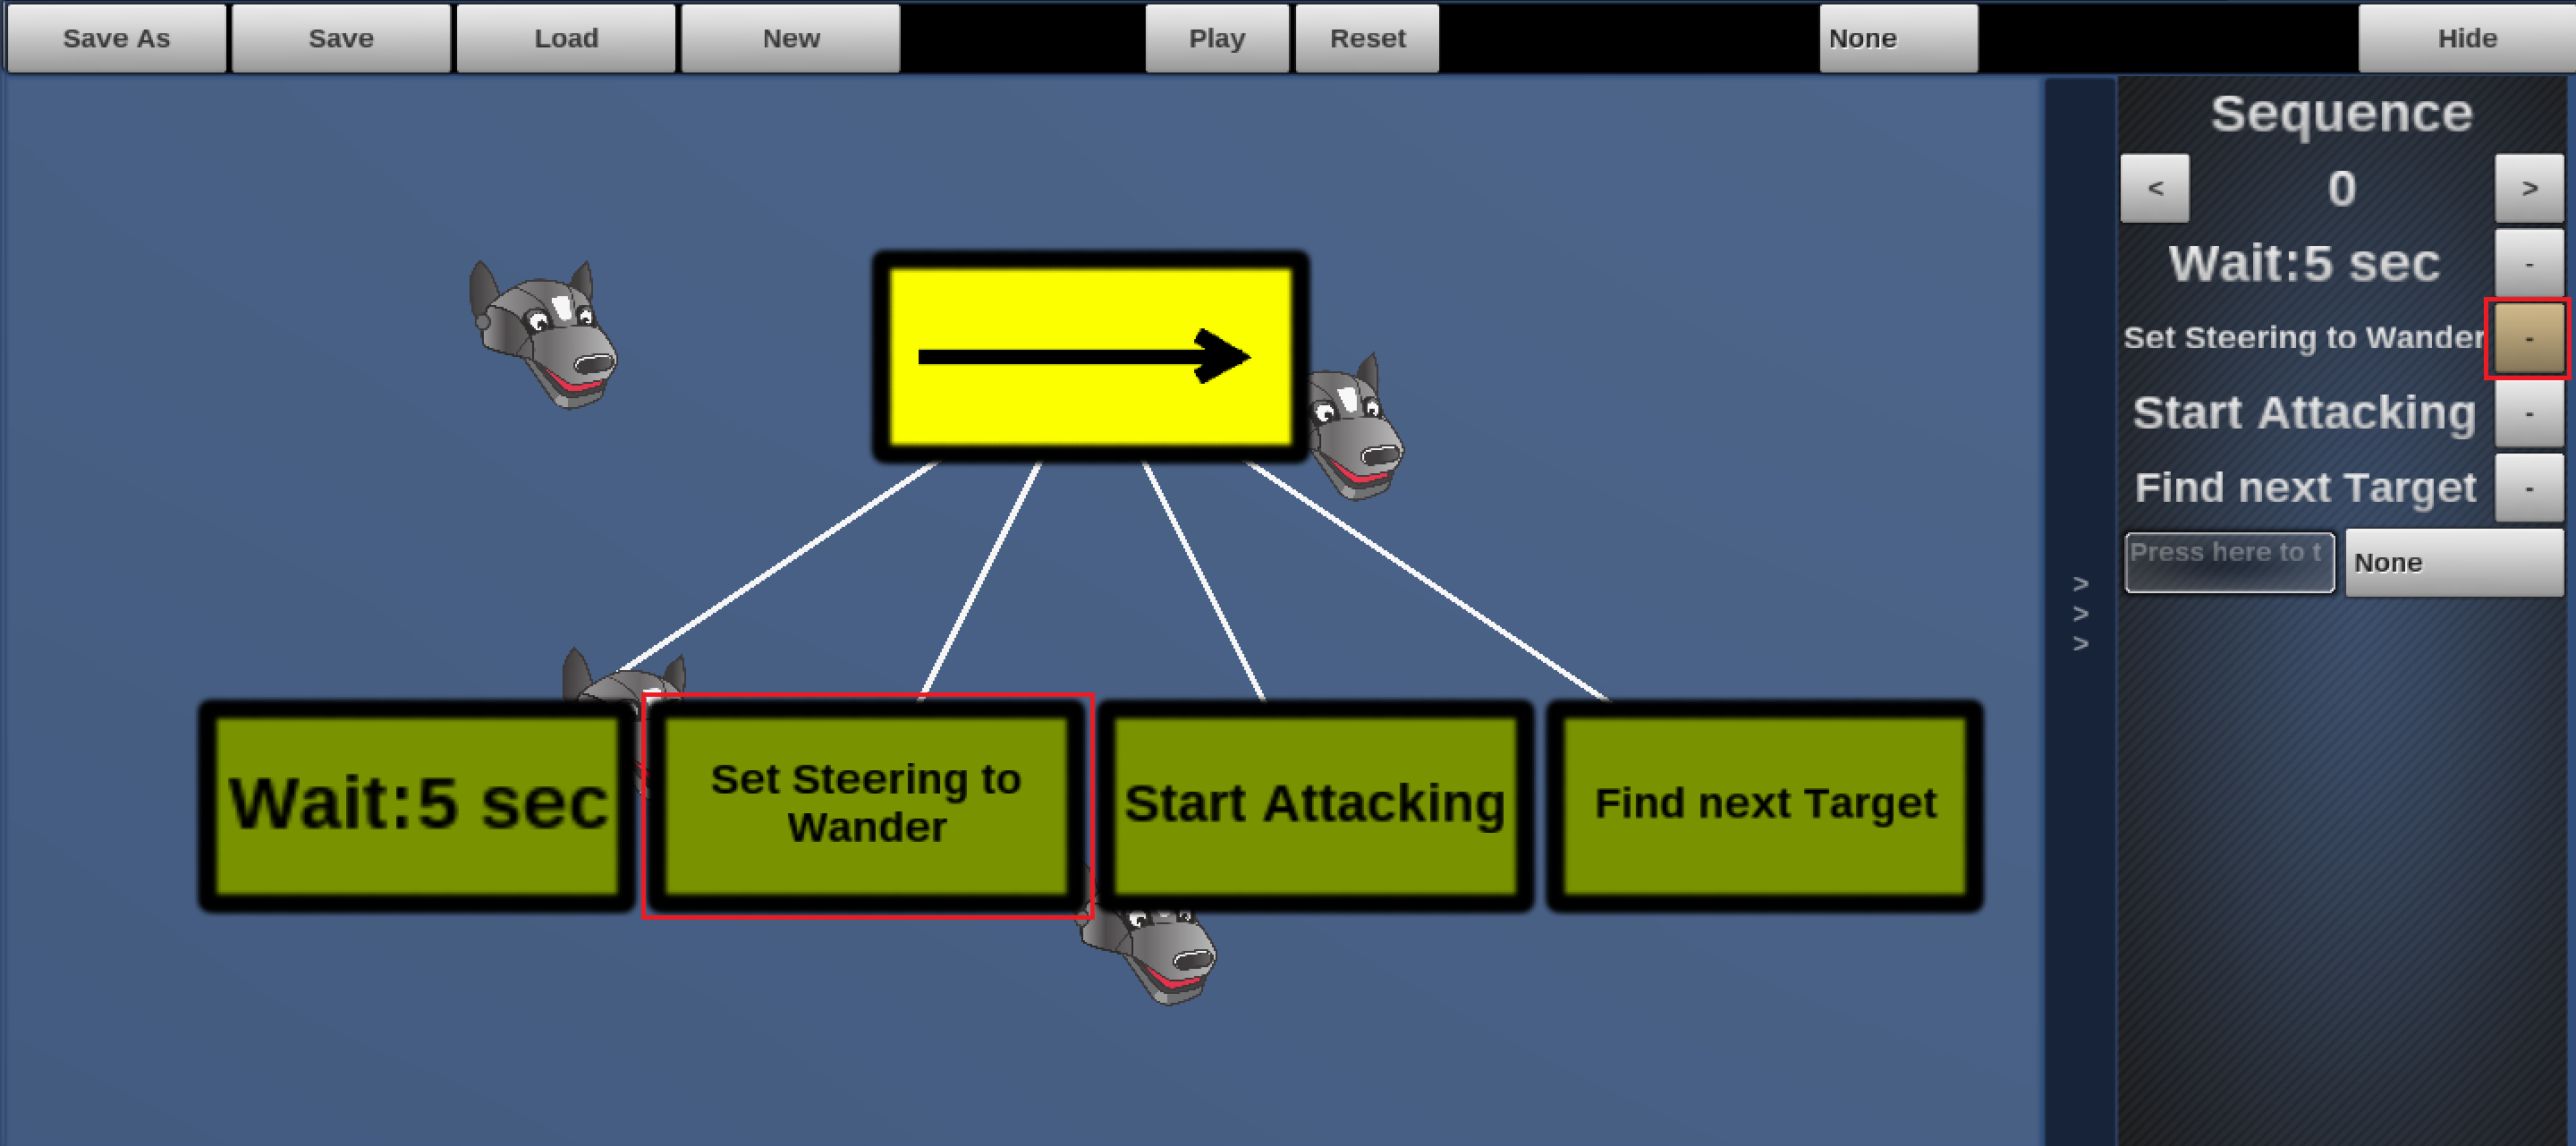
\includegraphics[width=1\textwidth]{images/KIAnleitung17_1}
	\caption{L�schen-Button Rechts neben dem Knotennamen}
	\label{a9}
\end{figure}

\begin{figure}[h!] %[hbtp]
	\centering
		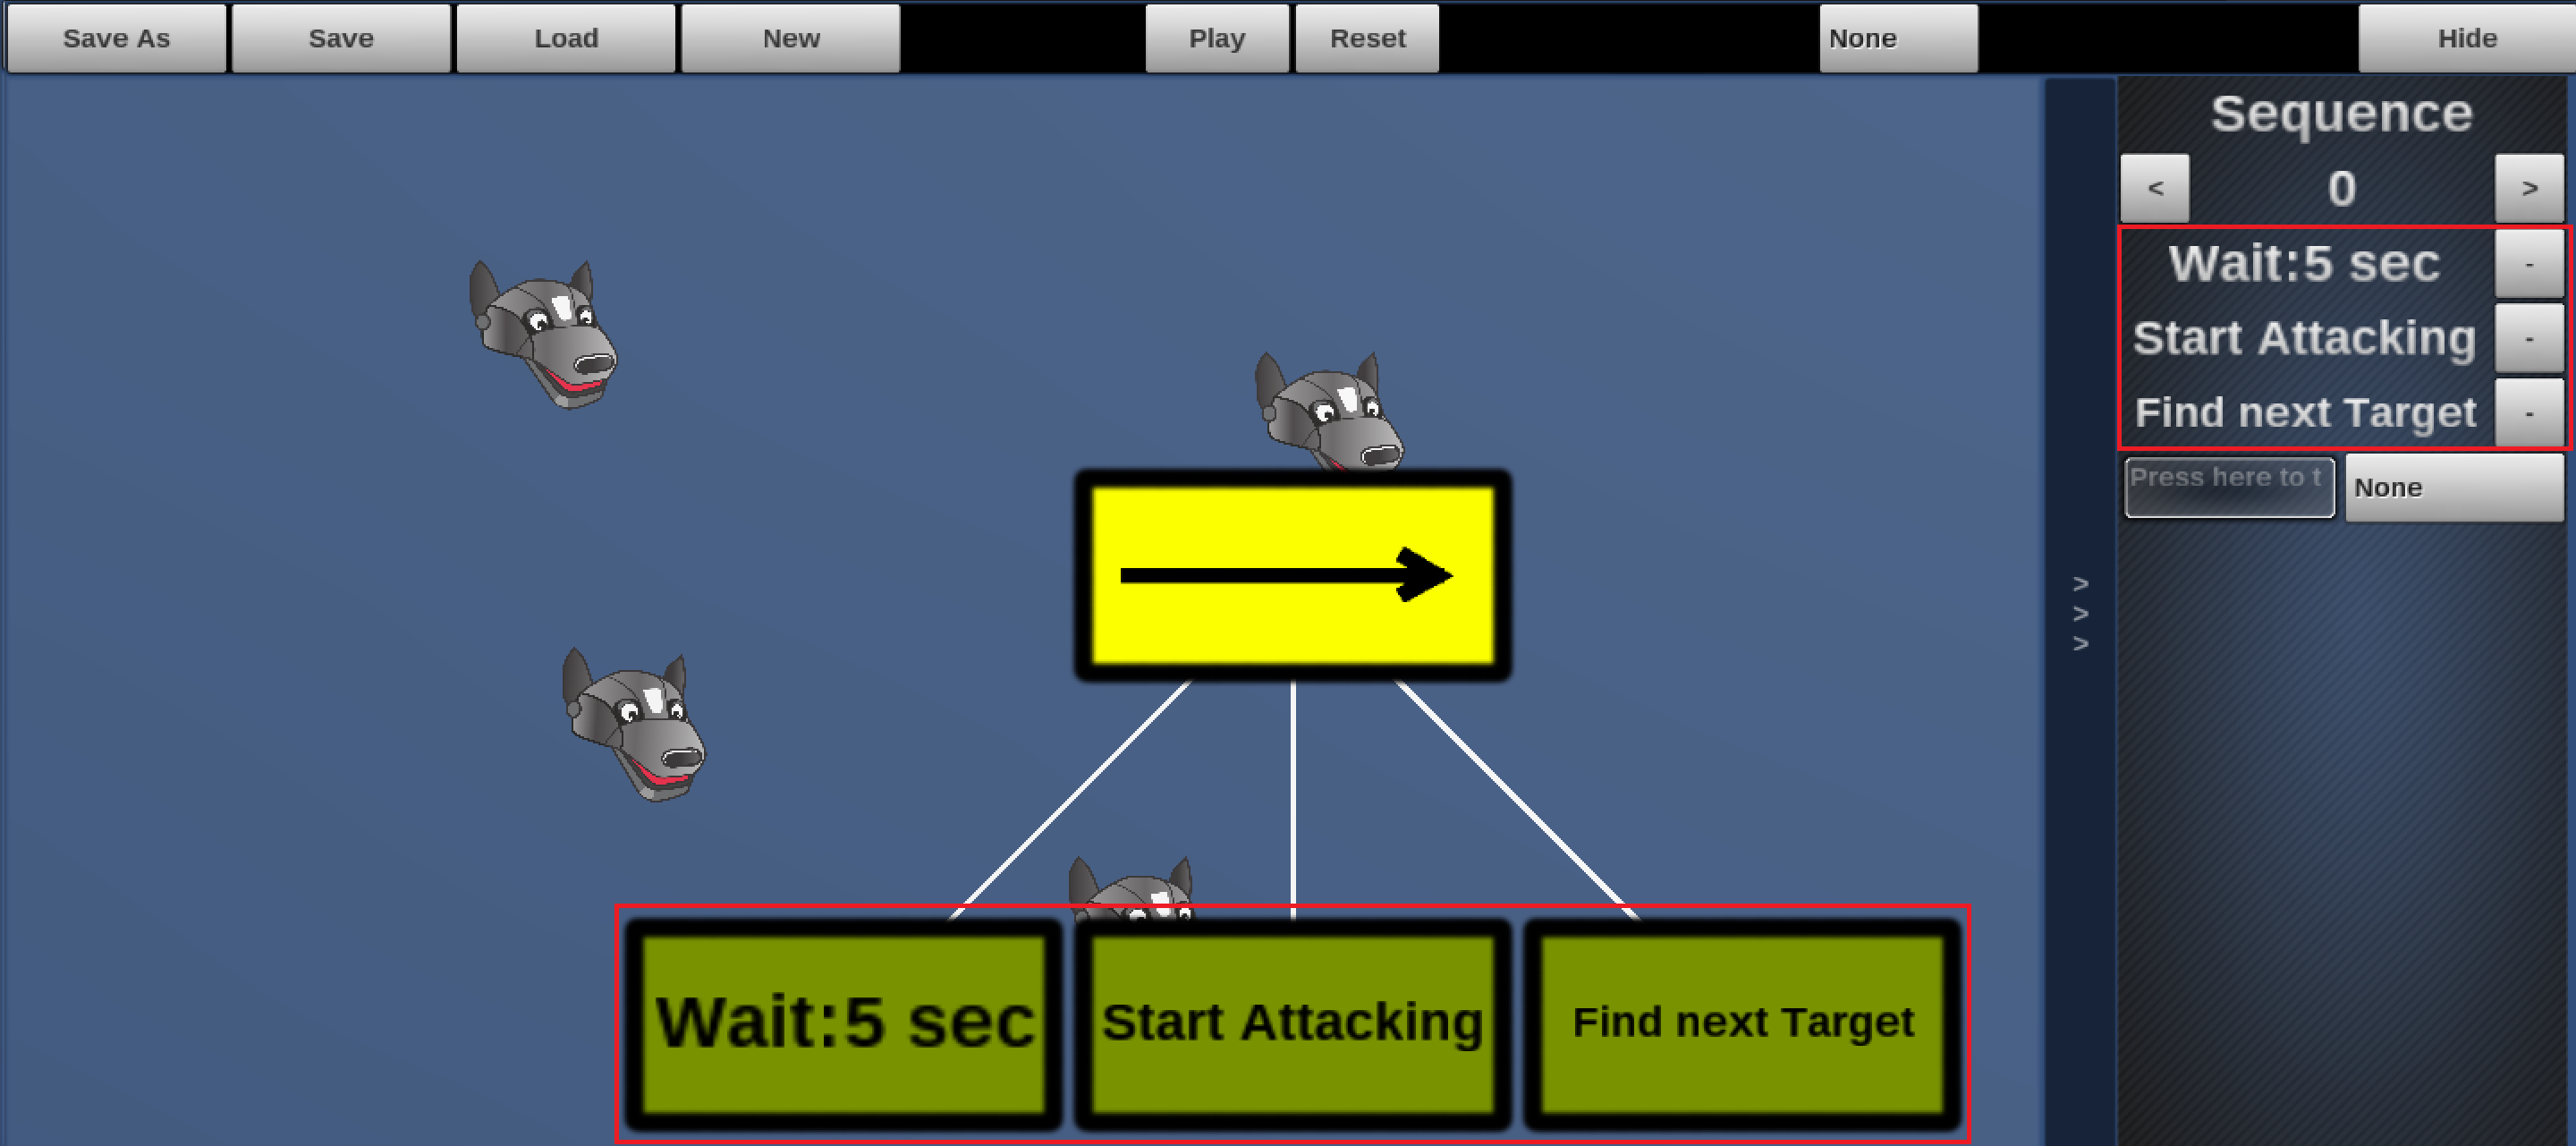
\includegraphics[width=1\textwidth]{images/KIAnleitung18_1}
	\caption{Der zu l�schende Kindknoten wurde gel�scht}
	\label{a10}
\end{figure}



\section{Speichern}
\subsection{Neuer Baum}
Beim Speichern eines neuen Baumes wird in der Leiste am oberen Bildschirmrand der "'Save As"'-Button ausgew�hlt. Dadurch �ffnet sich ein Fenster, in welchem der Name f�r den Baum eingegeben wird. Durch "'Save"' wird der Baum abgespeichert.

\begin{figure}[h!] %[hbtp]
	\centering
		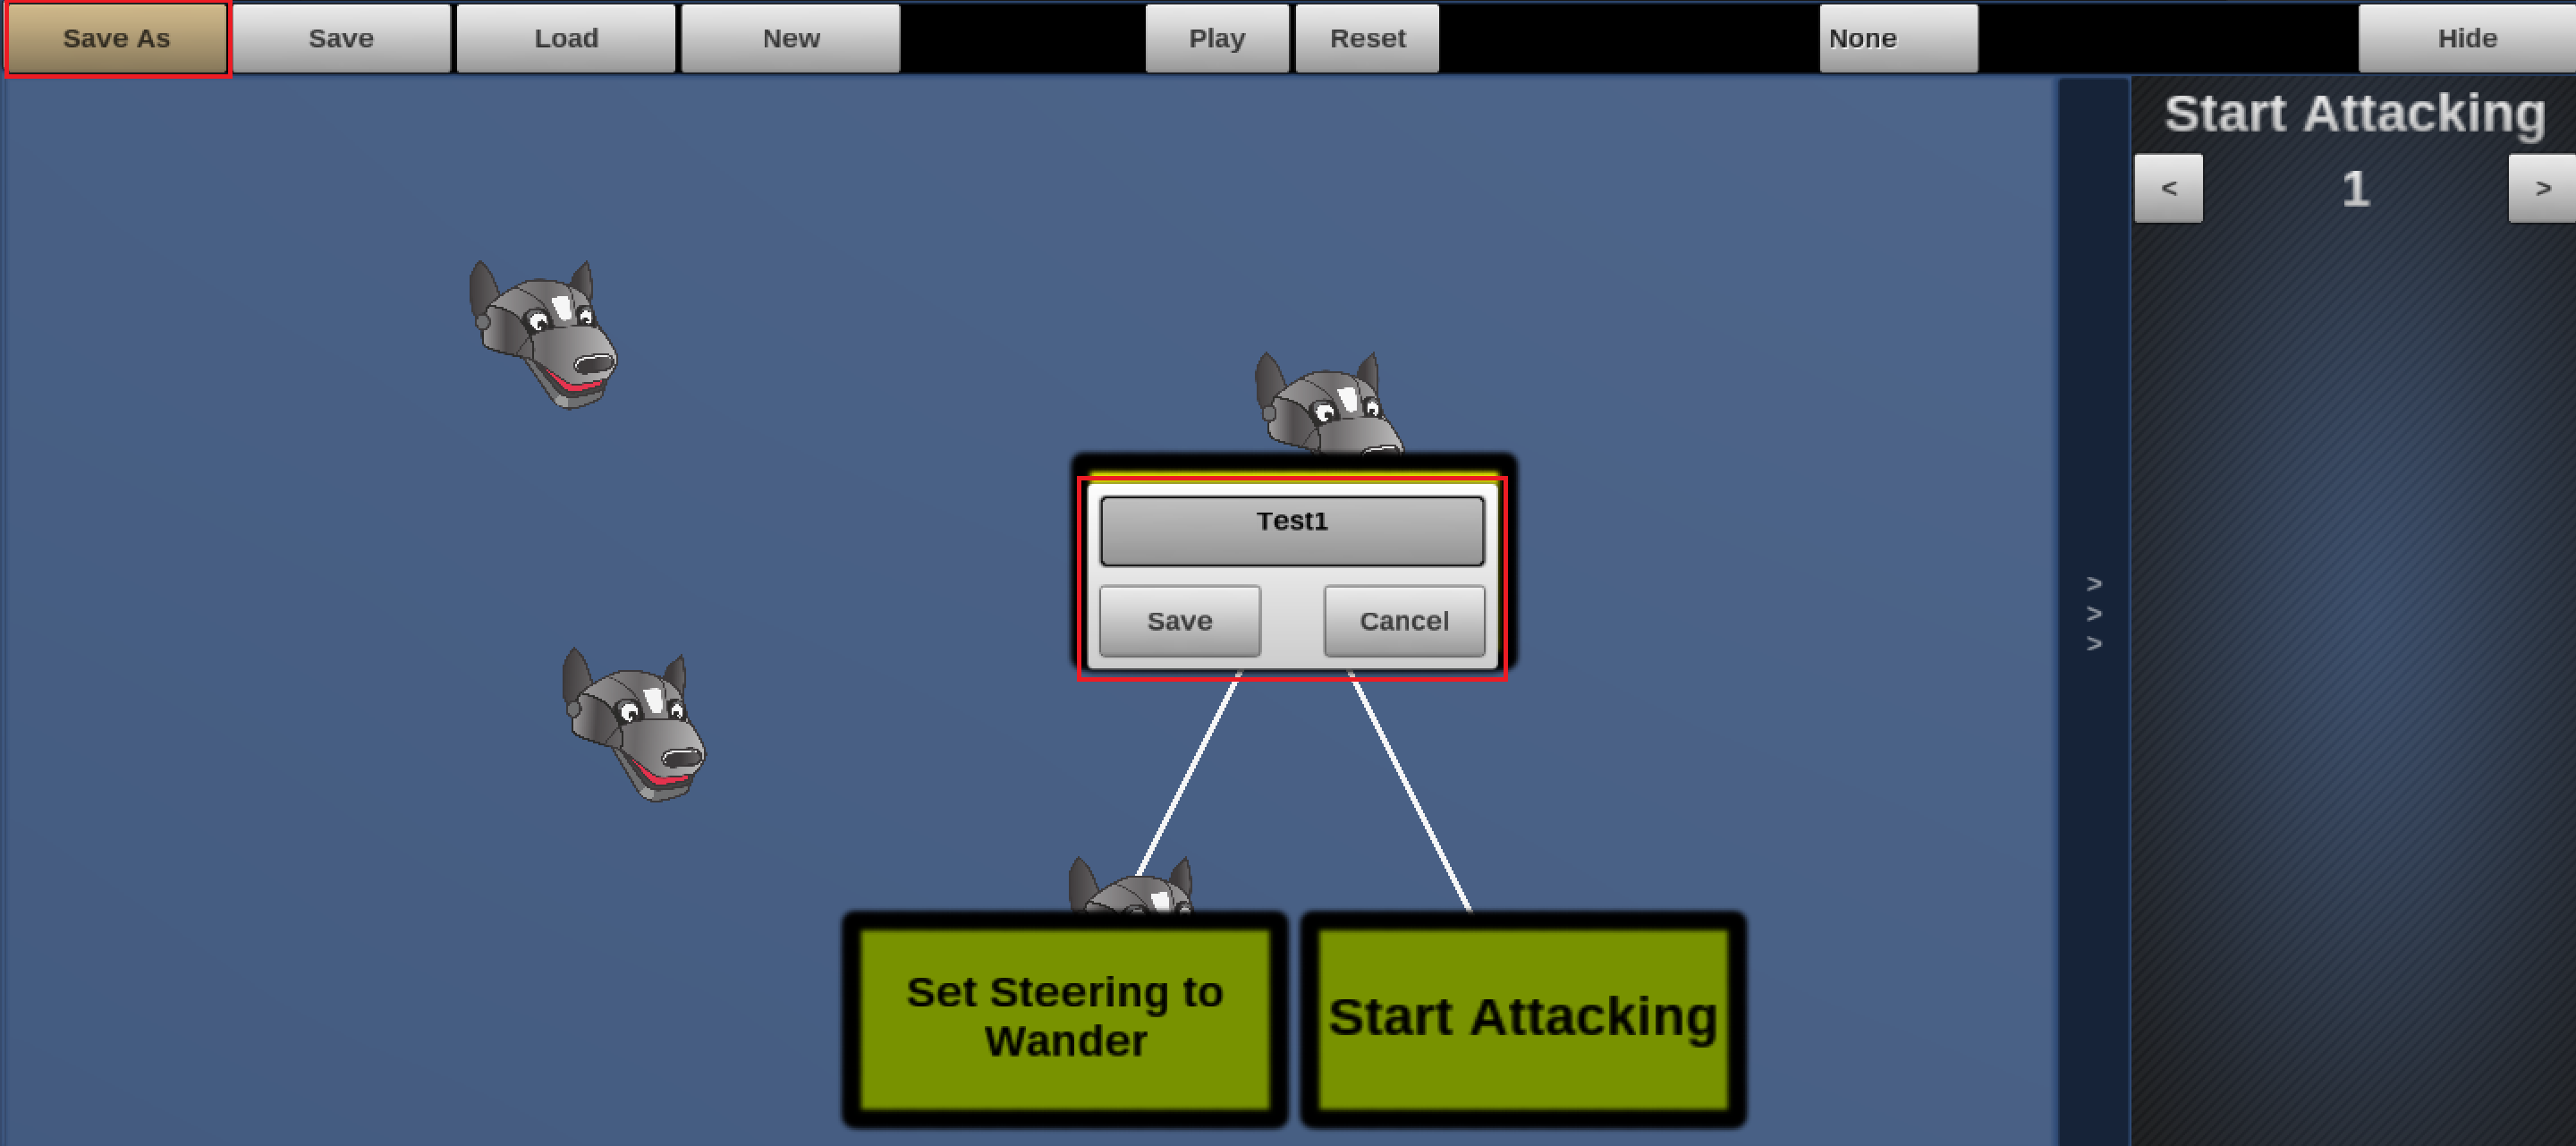
\includegraphics[width=1\textwidth]{images/KIAnleitung8_1}
	\caption{Neuer Baum wird durch Namensgebung abgespeichert}
	\label{a11}
\end{figure}
\subsection{Bereits vorhandener Baum}
Wenn ein bereits gespeicherter Baum ver�ndert wurde, kann der Fortschritt durch den Save-Button gesichert werden.

\begin{figure}[h!] %[hbtp]
	\centering
		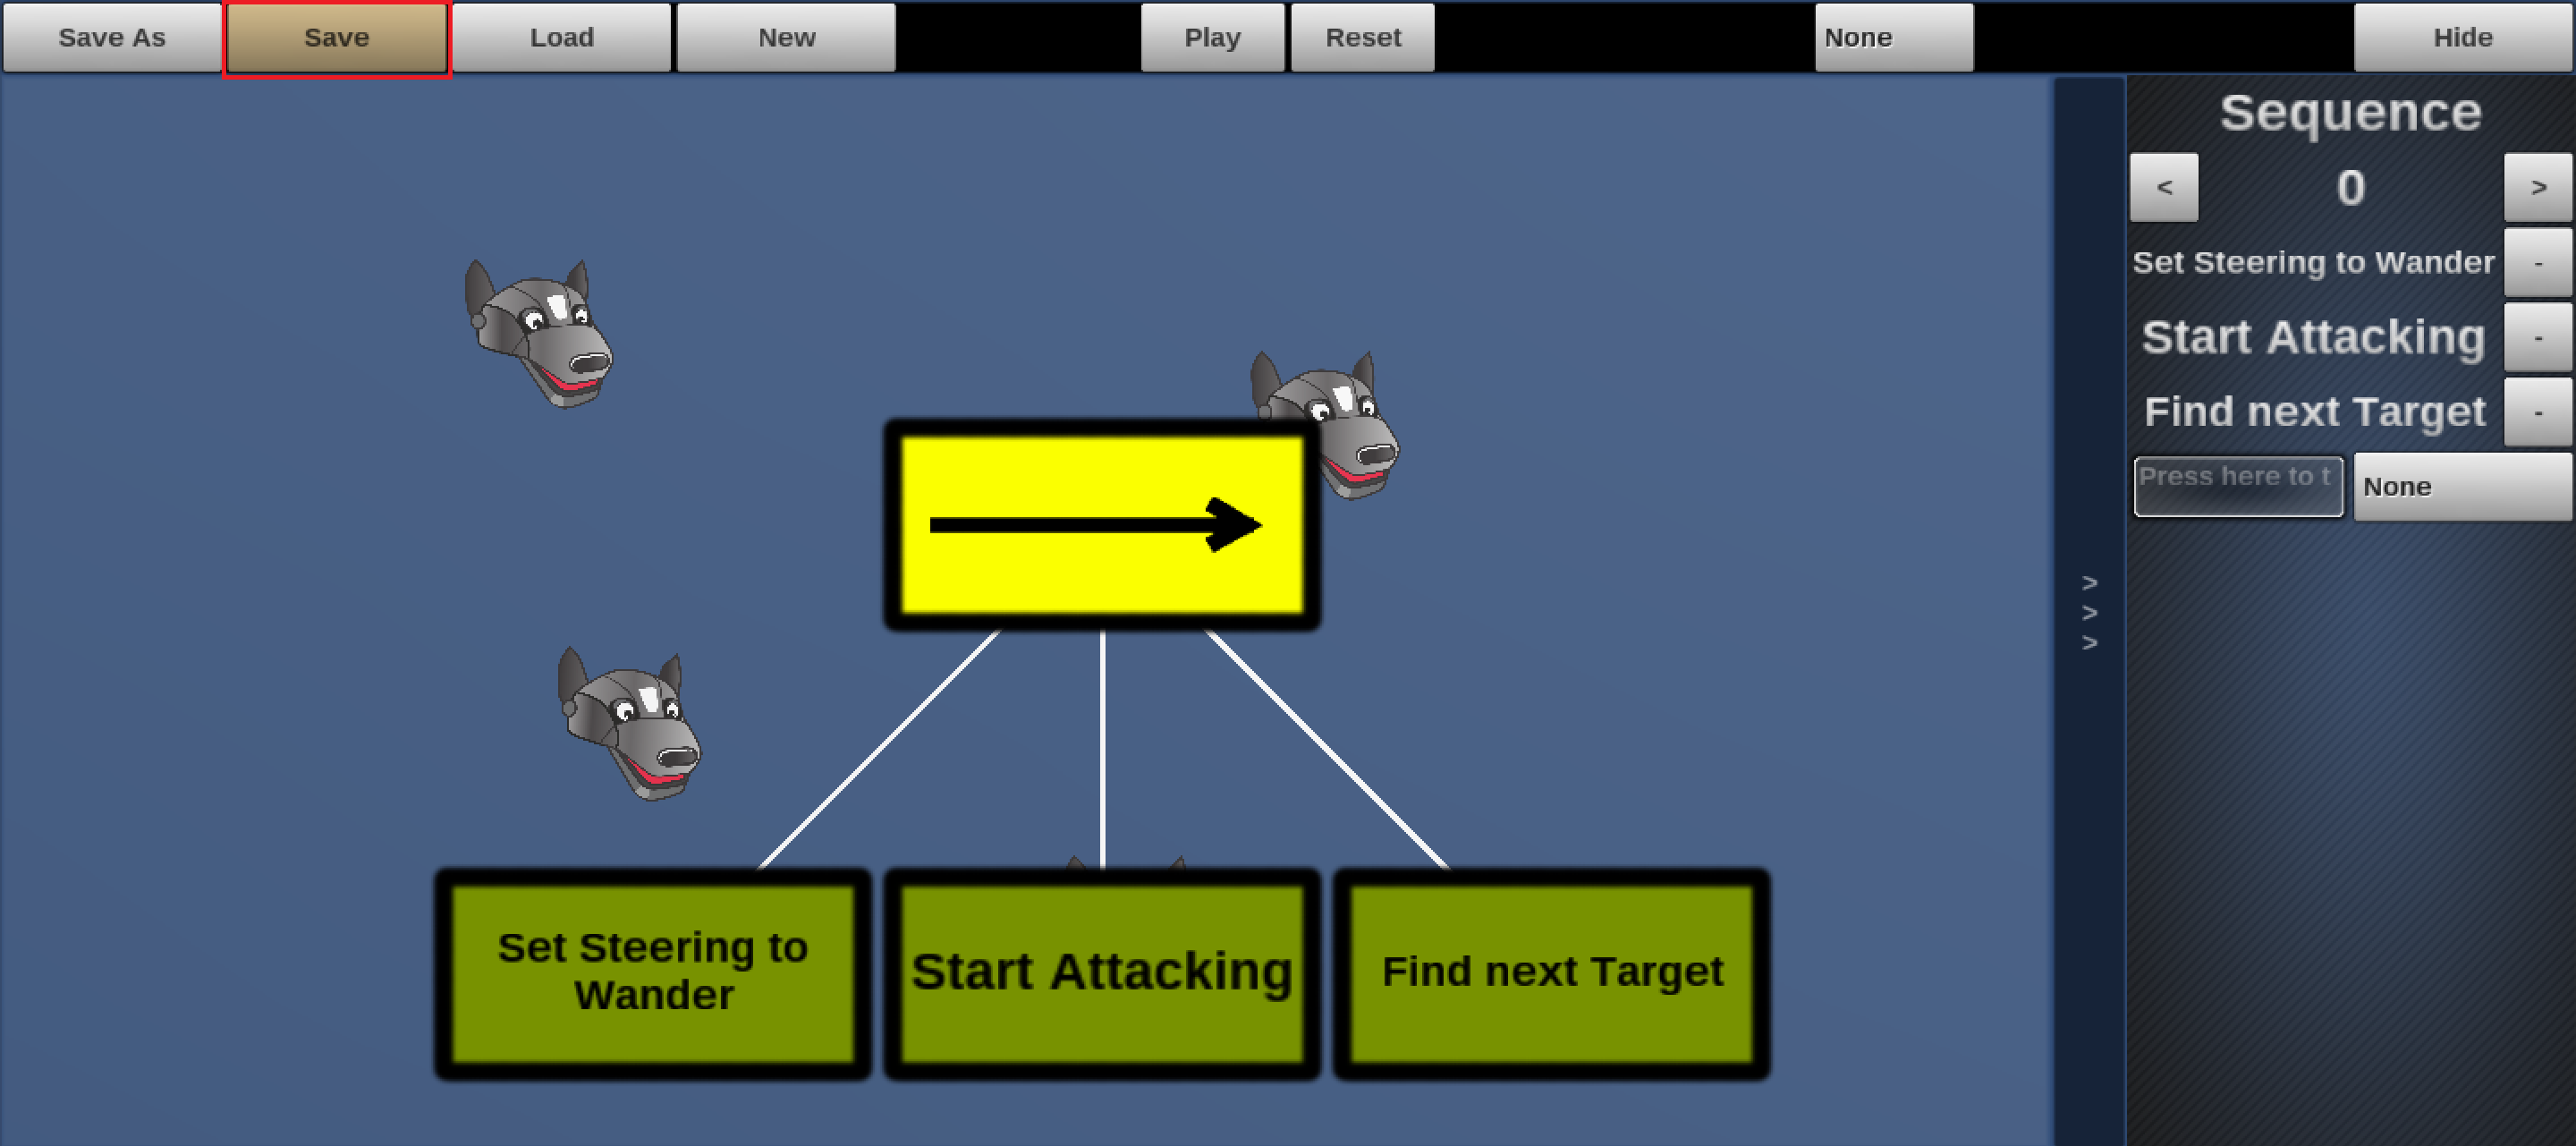
\includegraphics[width=1\textwidth]{images/KIAnleitung9_1}
	\caption{Bereits vorhandener Baum wird �berschrieben}
	\label{a12}
\end{figure}


\section{Laden}
�ber den Load-Button am oberen Bildschirmrand kann ein Baum aus einer Liste der gespeicherten B�ume ausgew�hlt werden, um diesen weiter zu editieren. 
\begin{figure}[h!] %[hbtp]
	\centering
		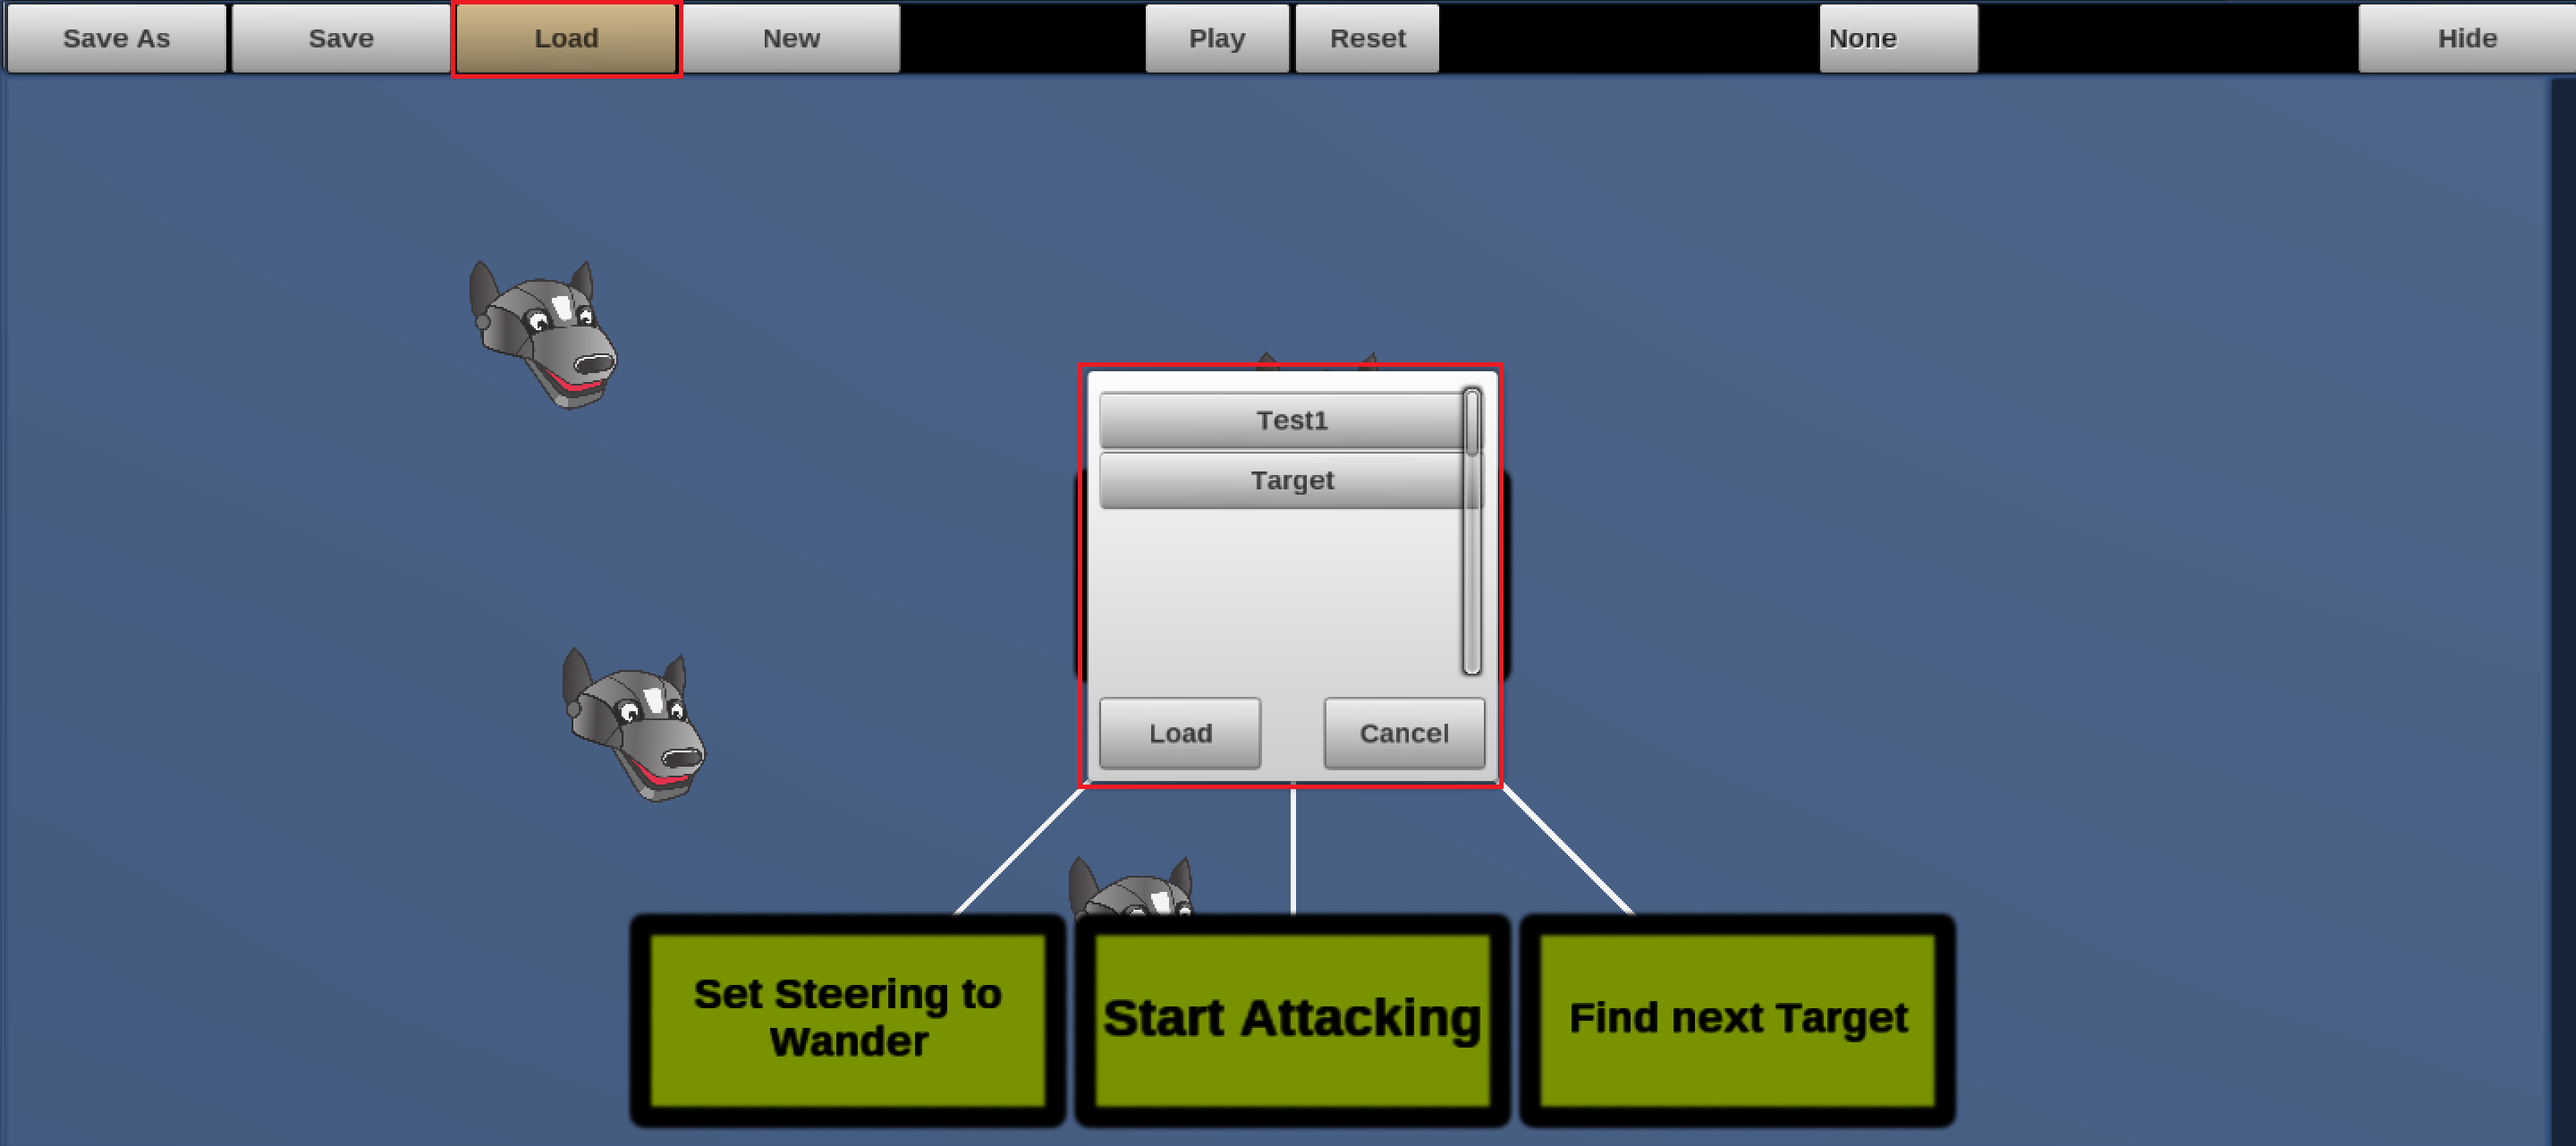
\includegraphics[width=1\textwidth]{images/KIAnleitung10_1}
	\caption{Liste mit bereits gespeicherten B�umen}
	\label{a13}
\end{figure}

\newpage
\section{Ablauf des Baumes verfolgen}
Um den Ablauf eines Baumes sehen zu k�nnen, muss bereits mindestens ein Roboter mit einem Behaviour Tree ausgestattet sein. Beim Klick auf den Button mit der Aufschrift "None" �ffnet sich die Liste mit Robotern, welchen bereits ein Baum zugewiesen wurde. Sobald dort ein solcher ausgew�hlt ist, werden die anderen Funktionen des Show-Modus automatisch deaktiviert und der zugeh�rige Baum taucht auf. Sobald das Szenario gestartet wird, werden aktuelle Pfade gr�n markiert.
\begin{figure}[h!] %[hbtp]
	\centering
		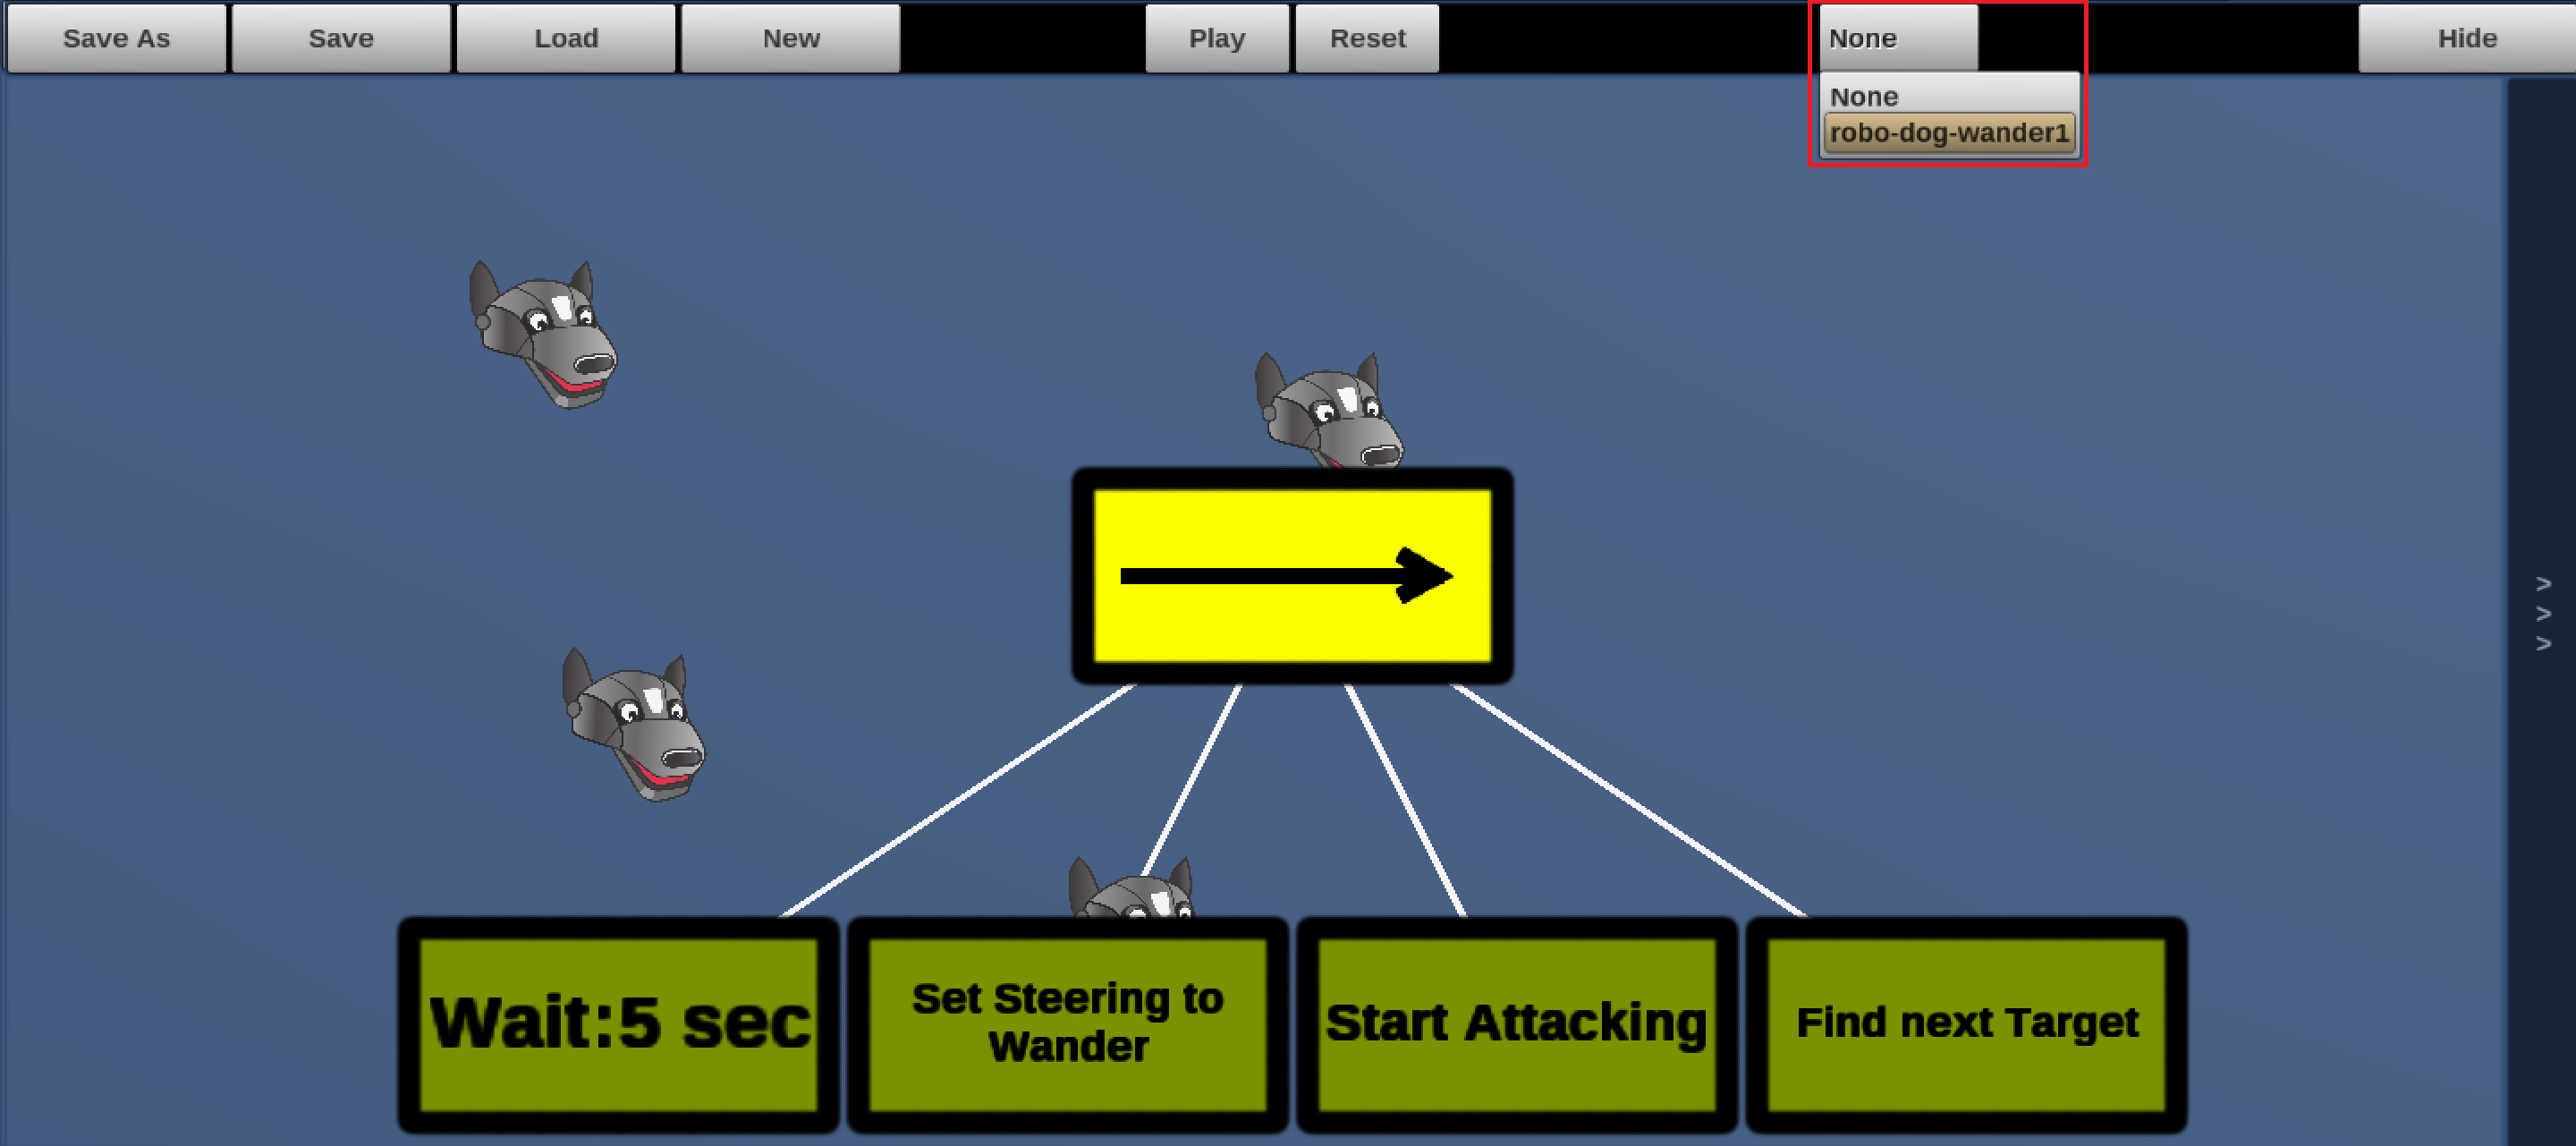
\includegraphics[width=1\textwidth]{images/KIAnleitung15_1}
	\caption{Auswahl eines Roboters}
	\label{a14}
\end{figure}

\begin{figure}[h!] %[hbtp]
	\centering
		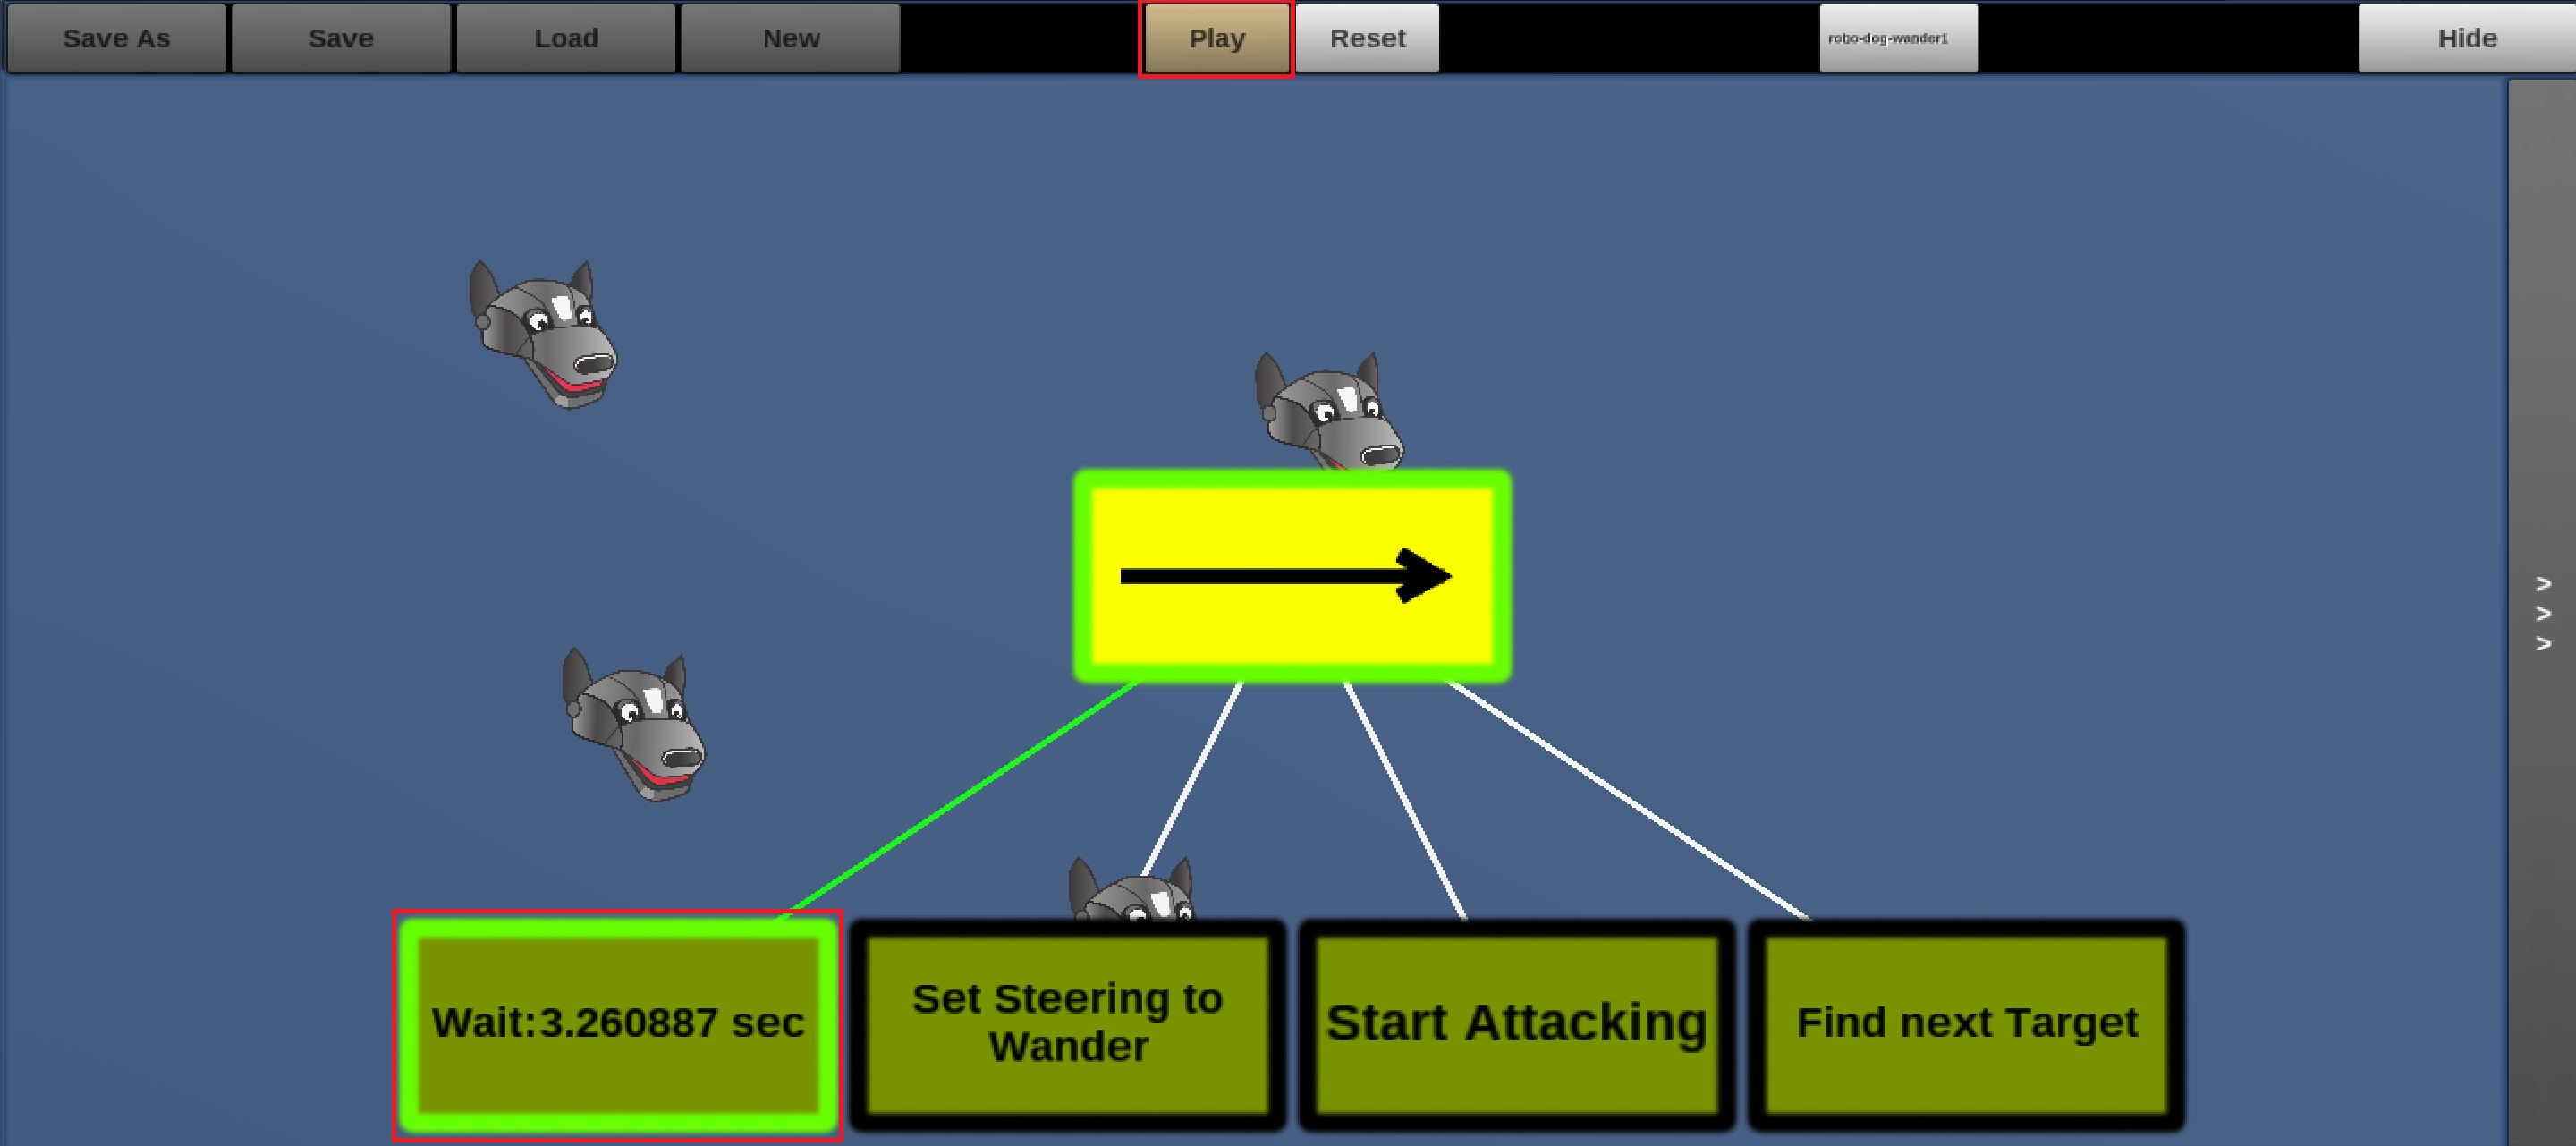
\includegraphics[width=1\textwidth]{images/KIAnleitung16_1}
	\caption{Aktuell ausgef�hrter Pfad im Behaviour Tree}
	\label{a15}
\end{figure}




\textbf{{\large Hide:}} Editor ist ausgeblendet.
Um den Baum-Editor zu verstecken bzw. auszuschalten, wird der Hide-Button gedr�ckt.

\section{Roboter einen Baum zuweisen}
Mit dem Rechtsklick der Maus auf einen beliebigen Roboter erscheint die Liste von bereits gespeicherten B�umen. Durch die Auswahl eines Baumes wird dieser dem Roboter zugeordnet.
\begin{figure}[h!] %[hbtp]
	\centering
		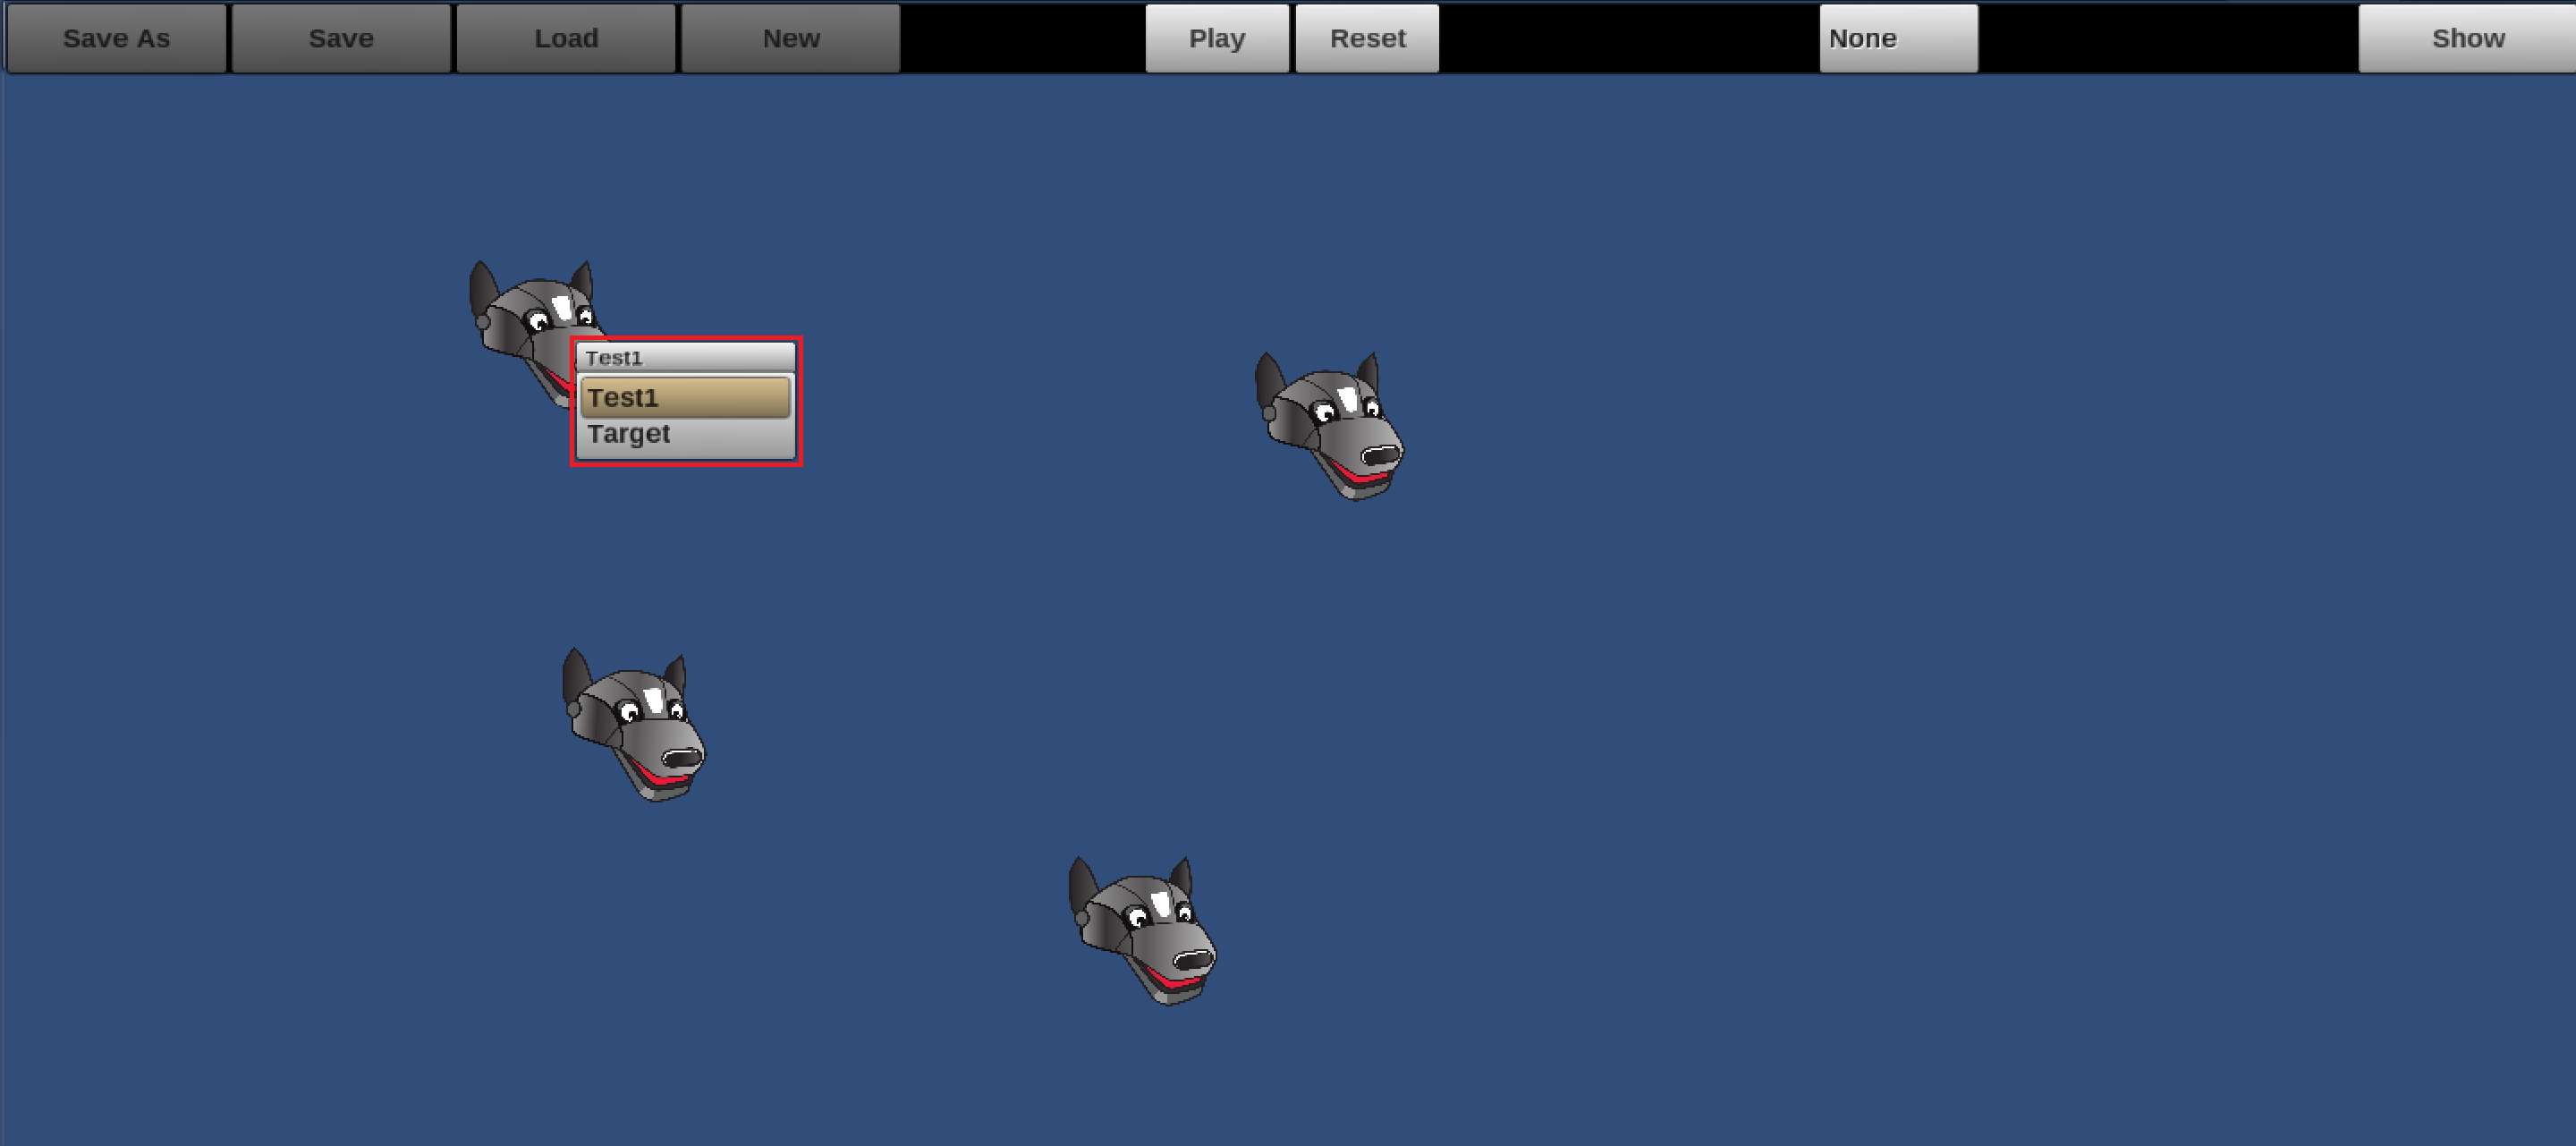
\includegraphics[width=1\textwidth]{images/KIAnleitung12_1}
	\caption{Einem Roboter wird ein Baum zugewiesen}
	\label{a16}
\end{figure}




\textbf{{\large Unabh�ngig von der Sichtbarkeit des Editors:}}

\section{Szenario Starten}
Durch das Dr�cken des Start-Buttons beginnt das Szenario. Alle zugewiesenen B�ume werden automatisch aktiviert.
\begin{figure}[h!] %[hbtp]
	\centering
		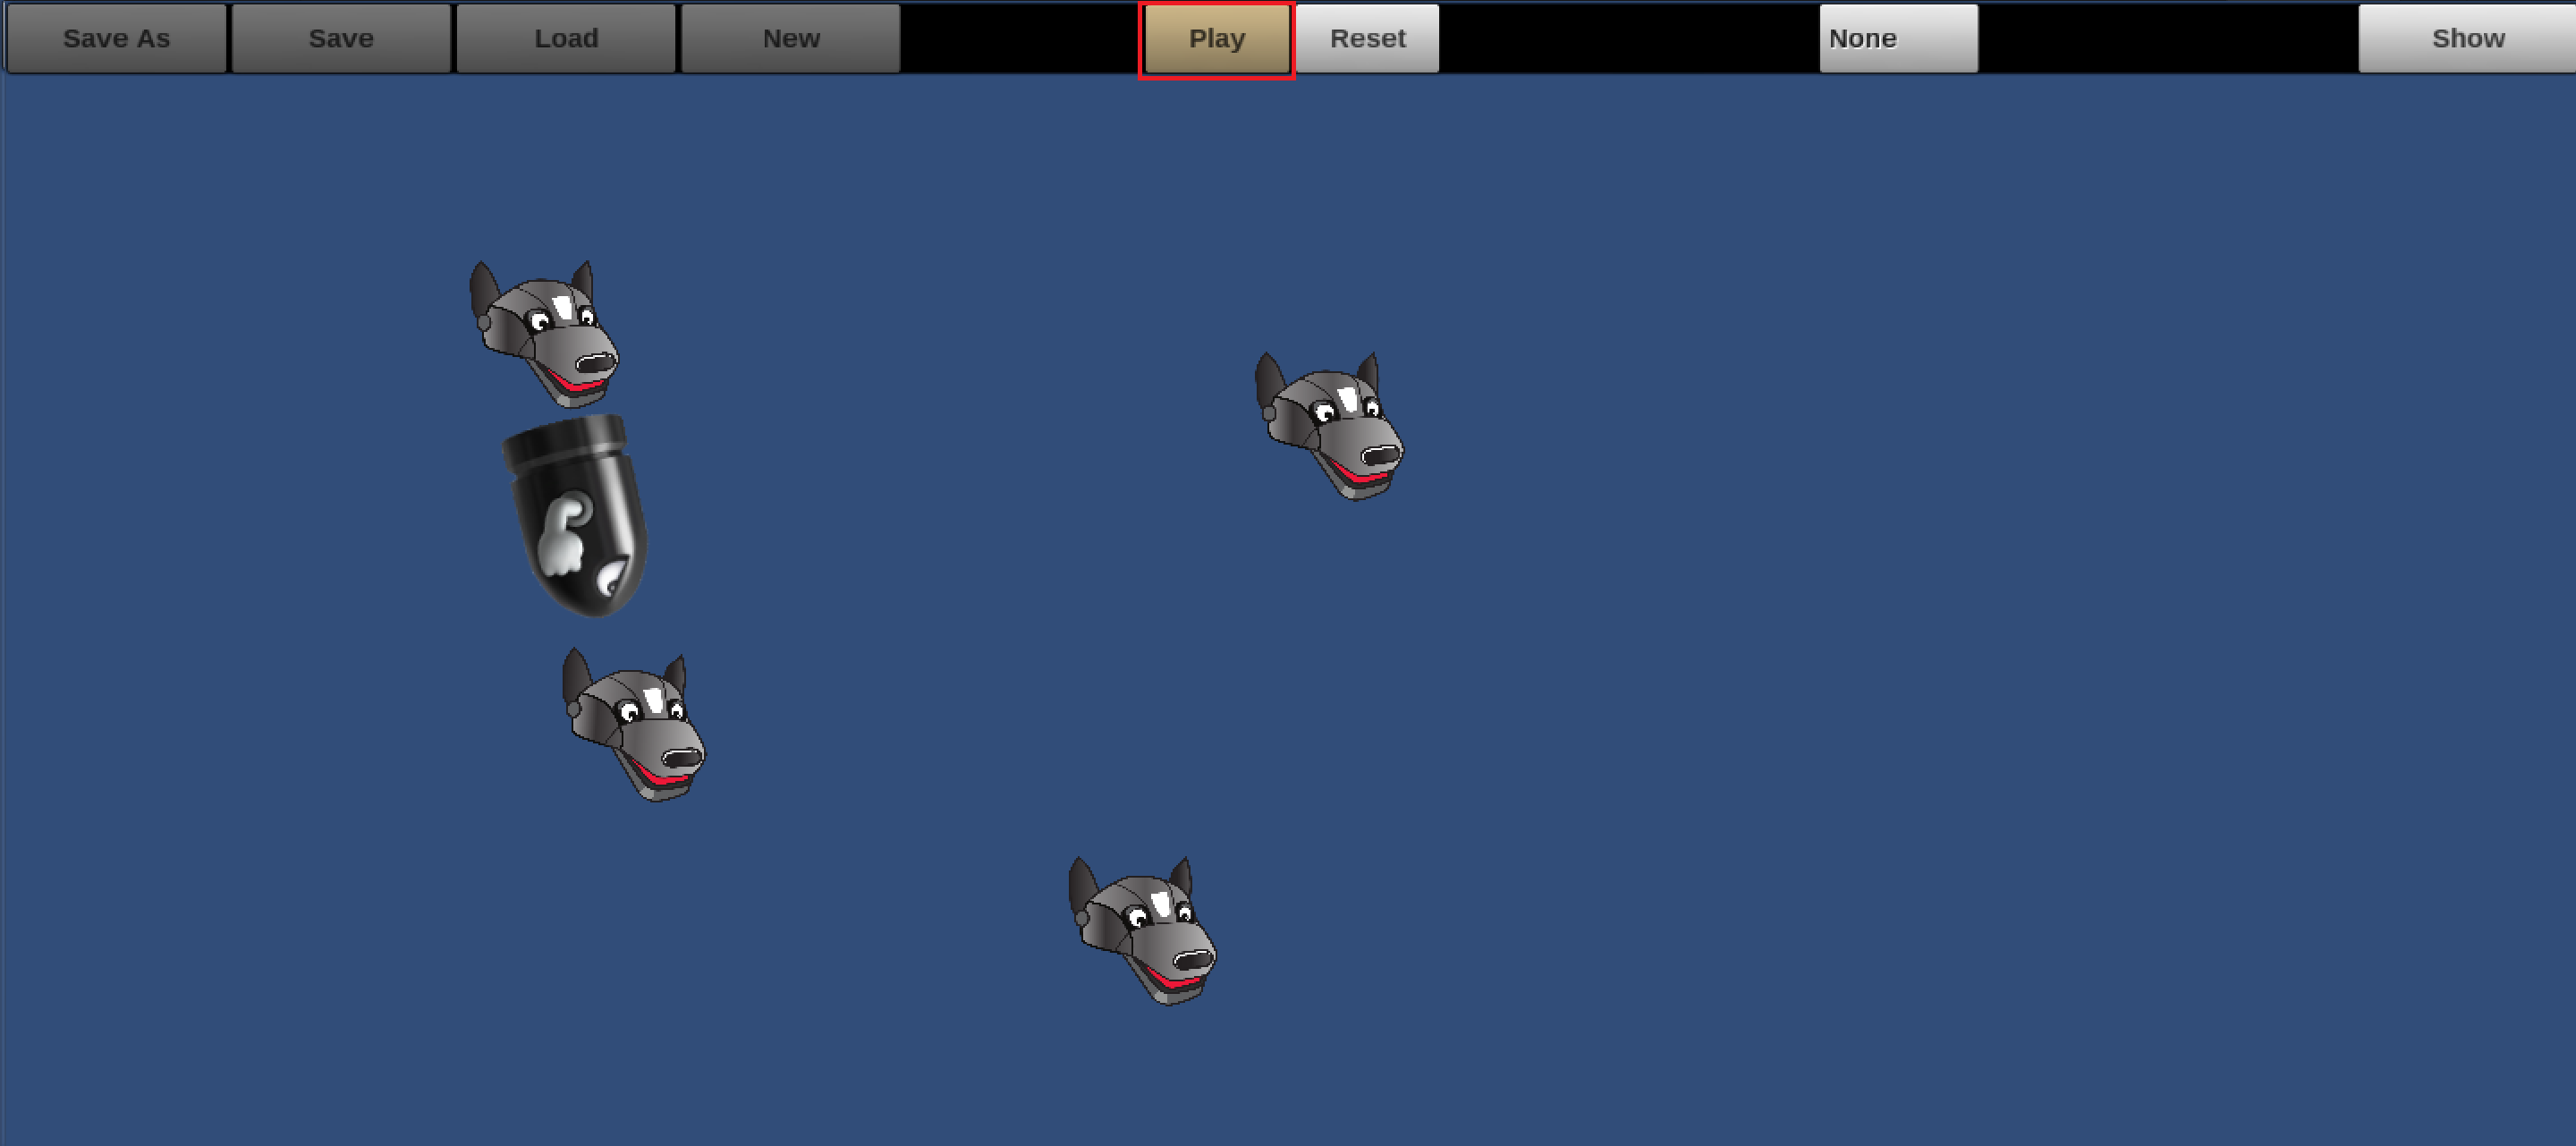
\includegraphics[width=1\textwidth]{images/KIAnleitung13_1}
	\caption{Ein aktuell laufendes Szenario}
	\label{a17}
\end{figure}



\section{Szenario zur�cksetzen}
Der Reset-Button kann jederzeit, w�hrend das Szenario l�uft, gedr�ckt werden. Alle Roboter werden auf Ihre Anfangsposition samt deren Anfangsattributwerte zur�ckgesetzt. Die zugewiesenen B�ume bleiben nach dem Reset erhalten.
\begin{figure}[h!] %[hbtp]
	\centering
		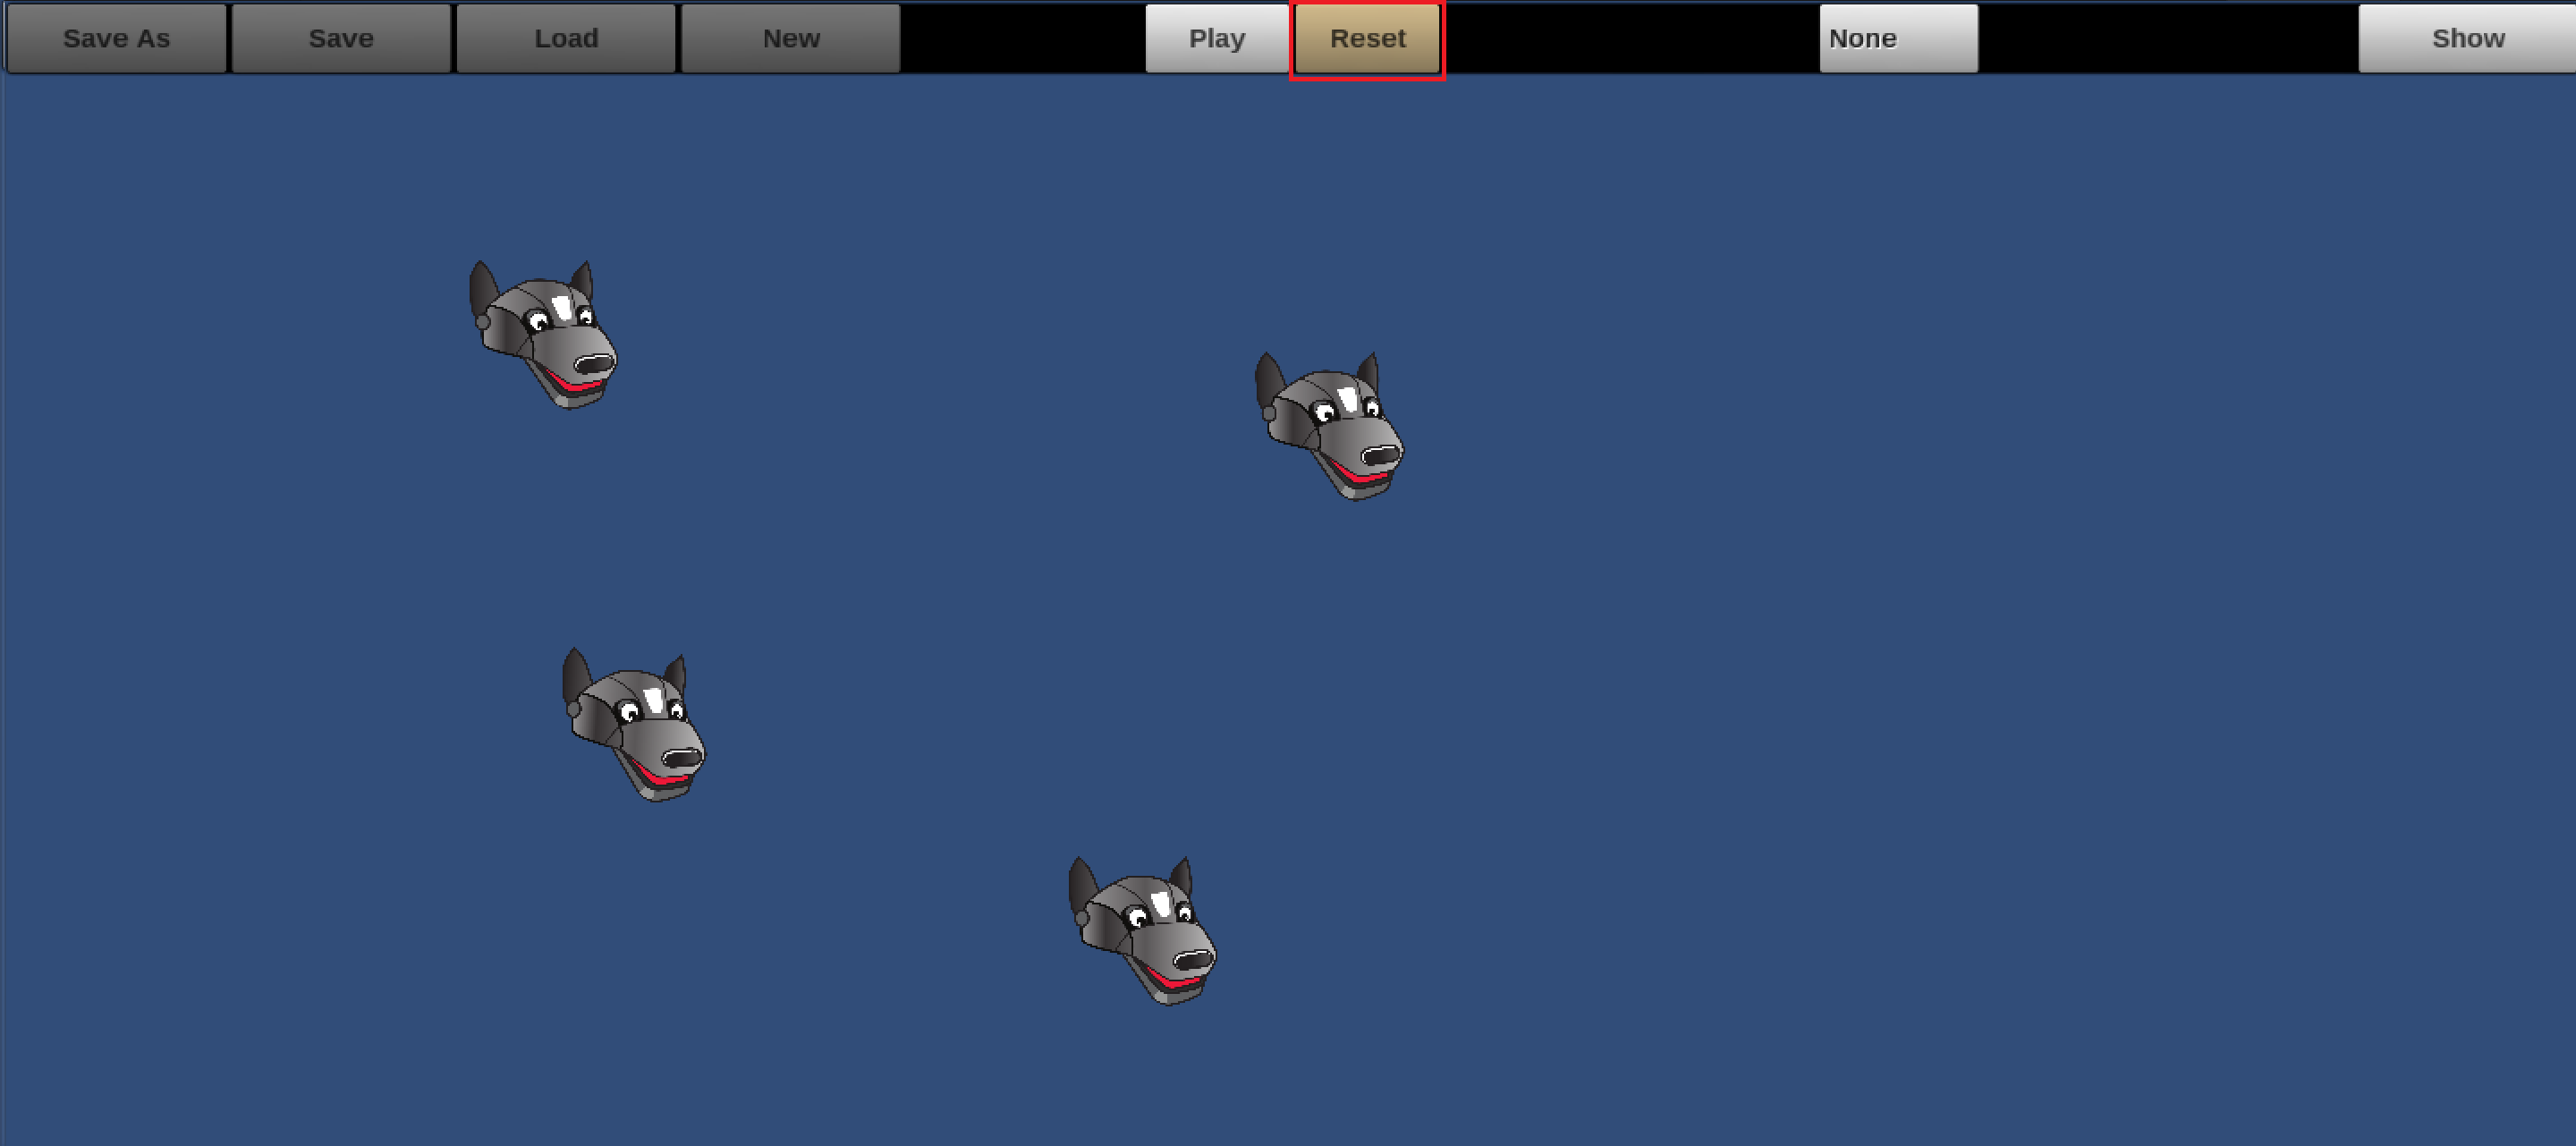
\includegraphics[width=1\textwidth]{images/KIAnleitung14_1}
	\caption{Nach Reset ist das Szenario in Ausgangsposition}
	\label{a18}
\end{figure}


